\documentclass{article}
\usepackage{graphicx}
\usepackage{amsmath, amssymb}
\usepackage{booktabs}
\usepackage{xcolor}
\usepackage{hyperref}
\usepackage{algorithm}
\usepackage{algpseudocode}
\usepackage{enumitem}
\usepackage{multirow}
\usepackage{array}
\usepackage{tikz}
\usetikzlibrary{arrows.meta}
\usepackage[edges]{forest}
\usepackage[textwidth=16cm, textheight=24cm]{geometry}
% ------------------------------------------------------------------
% Draft markers (redefine as no-ops for submission)
%   \citeneeded{...}  -> red    [CITE: ...]
%   \doubt{...}       -> blue   [DOUBT: ...]
%   \notetoself{...}  -> teal   [NOTE: ...]
%   \needresults{...} -> orange [RESULTS NEEDED: ...]
% ------------------------------------------------------------------
\newcommand{\citeneeded}[1]{\textcolor{red}{\textbf{[CITE: #1]}}}
\newcommand{\doubt}[1]{\textcolor{blue}{\textbf{[DOUBT: #1]}}}
\newcommand{\notetoself}[1]{\textcolor{teal}{\textit{[NOTE: #1]}}}
\newcommand{\needresults}[1]{\textcolor{orange}{\textbf{[RESULTS NEEDED: #1]}}}
\newcommand{\isa}{\texttt{IS\_A}}
\newcommand{\Mhero}{M_{\mathrm{HERO}}}

\title{Preserving the Meaning of Rare Clinical Concepts:\\ Ontology Tokenization by Distance-Aware Greedy Coverage}
\author{Yuanyuan Zheng}
\date{}

\begin{document}

\maketitle

\begin{abstract}
Foundation models trained on electronic health records (EHRs) usually give every clinical code its own embedding.
Because code usage is long-tailed, most codes are too rare for their embeddings to be learned, and frequency-based vocabulary truncation discards them; either way, the meaning of rare concepts is poorly learned or lost.
We propose a tokenizer that represents every concept of an ontology structured as a directed acyclic graph with a small vocabulary of the ontology's own concepts, chosen to preserve the meaning that the ontology states for them.
Tokens are selected by lazy greedy maximization of a semantic coverage objective whose credit decays with each hop, and each concept is written as a context tree that records through which relationship each token is reached.
We measure this ontology-based meaning with a proximity-coverage score that weights each branch of a concept's definition, together with uniqueness, unknown rate and length.
On 46,150 SNOMED~CT concepts mapped at a university hospital, our method with a decay of $\lambda = 0.9$ ranked first among 19 configurations at every compression level, ahead of degree-, centrality- and set-cover-based selections.
Applied to 279 million clinical events, a vocabulary of 5,000 tokens represented all 16,370 concepts of the data, including the two thirds that are rare and that frequency truncation discards entirely, with a mean proximity-coverage score of 0.88 for these rare concepts.
In a blinded comparison with the closest baseline, semanticians \needresults{preferred our representations for X\% of the concepts}.
Ontology-driven tokenization thus yields compact, auditable vocabularies in which rare concepts are expressed through tokens shared with frequent concepts, with limited loss of meaning.
\end{abstract}

\section{Introduction}
\label{sec:introduction}

Foundation models trained on electronic health records (EHRs) learn from long sequences of coded clinical events, such as diagnoses, procedures, prescriptions and laboratory tests, and can then be adapted to many downstream tasks \cite{li2020behrt, yang2023transformehr}.
These events are coded with standardized vocabularies, such as ICD, RxNorm, LOINC and SNOMED~CT, which make data comparable across institutions.

Most of these models give every code its own embedding, learned only from the occurrences of that code.
Code usage, however, is long-tailed \cite{zhang2023longtailed}: a few codes produce most events, and most codes are rare.
The embeddings of rare codes are therefore poorly learned \cite{gowda2020finding, land2024fishing}.
The common remedy, keeping only the $k$ most frequent codes and mapping the others to an unknown token, removes the rare codes altogether.
Either way, the meaning of rare concepts, which include specific diagnoses and procedures that can matter clinically, is poorly learned or lost.

Yet the meaning of a rare concept is not unknown: clinical ontologies state it explicitly.
SNOMED~CT, for instance, is a directed acyclic graph (DAG) in which each concept is linked to its more general parents and to the values of its attributes, such as its finding site or its morphology.
A rare concept is thus related to more frequent concepts that describe parts of its meaning.
This suggests representing each concept with a small vocabulary of ontology concepts, chosen so that every concept keeps as much of its meaning as possible.

Existing vocabulary strategies do not do this (Table~\ref{tab:related-approaches}).
Data-driven vocabularies ignore the ontology: the full vocabulary leaves rare codes under-trained, frequency truncation drops them, and subword methods such as Byte-Pair Encoding \cite{sennrich2016bpe, kudo2018sentencepiece}, adapted to code sequences \cite{unistruct}, merge codes by co-occurrence, which reflects local coding practice rather than clinical meaning.
Ontology-guided methods use the hierarchy but lose information or auditability.
Roll-up replaces rare codes with a broader ancestor and merges distinct subtypes \cite{redekop2025zeroshot}.
Splitting codes into prefix tokens \cite{renc2024ethos, waxler2025comet} works only when the identifier itself encodes the hierarchy, as in ICD-10 or ATC.
GRAM \cite{choi2017gram} keeps every code and borrows information from ancestors, but uses only parent--child edges.
MedTok \cite{su2025medtok} compresses codes into a learned codebook whose entries are latent vectors rather than clinical concepts \cite{vandenoord2017vqvae}.
Outside the clinical domain, NodePiece \cite{galkin2022nodepiece} encodes the nodes of a knowledge graph by a few anchor nodes, chosen by centrality, and ignores the relationships along the path to each anchor.
No existing strategy compresses the vocabulary while keeping every concept, the relationships that define it, and tokens that are themselves interpretable concepts.

\begin{table*}[t]
\centering
\small
\resizebox{\textwidth}{!}{%
\begin{tabular}{llccl}
\toprule
\textbf{Approach} & \textbf{Ontology used} & \textbf{Compresses} & \textbf{Auditable} & \textbf{Main limitation} \\
\midrule
Full vocabulary & none & \texttimes & \checkmark & rare codes under-trained \\
Frequency top-$k$ & none & \checkmark & \checkmark & rare concepts dropped \\
Subword / BPE \cite{sennrich2016bpe, unistruct} & none (co-occurrence) & \checkmark & \texttimes & order-dependent; reflects local coding practice \\
Hierarchy roll-up \cite{redekop2025zeroshot} & \isa{} only & \checkmark & \checkmark & distinct subtypes merged into a parent \\
Identifier prefix split \cite{renc2024ethos, waxler2025comet} & implicit (code syntax) & \checkmark & partial & needs hierarchical identifiers \\
GRAM \cite{choi2017gram} & \isa{} only & \texttimes & \checkmark & no compression; attributes ignored \\
MedTok \cite{su2025medtok} & graph and text & \checkmark & \texttimes & latent codebook, not human-readable \\
NodePiece \cite{galkin2022nodepiece} & general graph & \checkmark & partial & centrality anchors; relations on paths ignored \\
\midrule
\textbf{Ours} & \textbf{full DAG, all relationships} & \checkmark & \checkmark & longer sequences \\
\bottomrule
\end{tabular}%
}
\caption{Vocabulary strategies for EHR foundation models.}
\label{tab:related-approaches}
\end{table*}

We propose a tokenizer that fills this gap in two stages (Figure~\ref{fig:pipeline}).
First, it selects $k$ tokens among the concepts of the ontology by maximizing a \emph{semantic coverage} objective, in which the credit for reaching a token decays with each hop, since part of the meaning is lost at every hop.
Second, it writes each concept as a \emph{context tree} that records through which relationship each token is reached.
A rare concept is then expressed with tokens it shares with frequent, related concepts, while keeping the relationships that distinguish it from them.

\begin{figure*}[t]
\centering
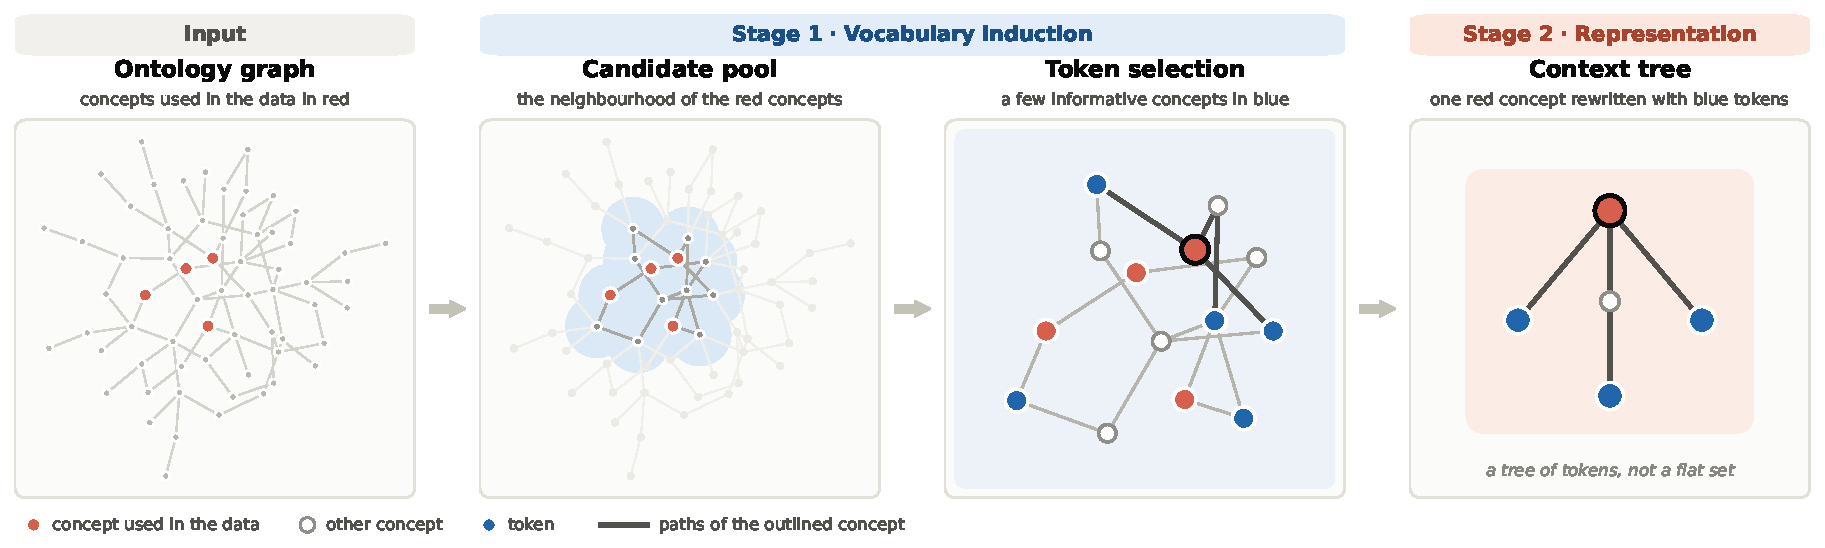
\includegraphics[width=\textwidth]{imgs/pipeline_illustration.pdf}
\caption{Overview of the two-stage pipeline on a toy ontology.
Input: an ontology graph in which the concepts used in the data are shown in red.
Stage~1 (vocabulary selection): candidate tokens are restricted to the neighbourhood of these concepts (Section~\ref{sec:method:candidates}), and a greedy selection picks a small set of tokens (blue) that best cover them (Sections~\ref{sec:method:score}--\ref{sec:method:selection}).
Stage~2 (context trees): each concept is rewritten as a tree over the tokens; the outlined concept reaches two tokens directly and a third through an intermediate concept, and keeps these paths rather than a flat set of tokens (Section~\ref{sec:method:tokenizer}).}
\label{fig:pipeline}
\end{figure*}

Our contributions are:
\begin{enumerate}[leftmargin=*, label=(\arabic*)]
    \item a formulation of vocabulary selection on a DAG ontology as the maximization of a distance-decayed semantic coverage, a monotone submodular objective solved by lazy greedy selection with a $(1 - 1/e)$ guarantee, whose decay can follow properties of the ontology such as the definition status of concepts (Section~\ref{sec:method});
    \item context trees, which keep the relationship through which each token is reached, and the proximity-coverage score, which weights each branch of a concept's definition and measures how much of the meaning stated by the ontology a tokenization preserves (Sections~\ref{sec:method:tokenizer}--\ref{sec:method:metrics});
    \item a benchmark on 46,150 SNOMED~CT concepts mapped at a university hospital, in which our method obtains the best average rank over four metrics, and a higher proximity-coverage score, at every compression level, against seven graph-based selections and a set-cover ablation, while using almost every token it selects (Section~\ref{sec:results:benchmark});
    \item an application to 279 million clinical events, in which a vocabulary of 5,000 tokens represents all 16,370 concepts of the data that are in the ontology graph, including the two thirds that are rare and that frequency truncation discards, with a mean proximity-coverage score of 0.88 for the rare concepts (Section~\ref{sec:results:hero});
    \item a blinded comparison by semanticians with the closest baseline (Section~\ref{sec:results:expert}).
\end{enumerate}

\section{Background: SNOMED~CT}
\label{sec:background}
\label{sec:snomed}

SNOMED~CT is the most comprehensive clinical terminology in use \cite{snomed2024starter}.
The release we use contains more than 420,000 concepts, covering disorders, procedures, substances, body structures and more, connected by 113 relationship types.
Concepts and relationships together form a DAG (Section~\ref{sec:method:problem}).

\paragraph{Hierarchy and attributes.}
Relationships are of two kinds.
An \isa{} relationship $u \xrightarrow{\isa} v$ states that $u$ is a subtype of $v$; a concept may have several parents, so the hierarchy is a polyhierarchy.
Every other relationship states the value of an attribute: $u \xrightarrow{R} v$, for $R$ such as \emph{finding site} or \emph{associated morphology}, means that the value of attribute $R$ for $u$ is $v$, not that $v$ is more general than $u$.
For instance, \emph{Neoplasm of bone of upper limb} is a neoplasm (its associated morphology) located in the bone of the upper limb (its finding site), and a subtype of \emph{Neoplasm of bone} and of \emph{Structural abnormality of upper limb bone} (Figure~\ref{fig:shared-structure}).
Our tokenizer treats the two kinds of edge differently (Section~\ref{sec:method:tokenizer}).

\paragraph{Shared meaning.}
Because meaning is carried by edges, two distinct concepts share part of their meaning when they reach the same concepts through the same relationships.
\emph{Fracture of upper limb} and \emph{Neoplasm of bone of upper limb} are different disorders, yet both are subtypes of \emph{Structural abnormality of upper limb bone} and both have \emph{Bone structure of upper limb} as their finding site (Figure~\ref{fig:shared-structure}).
This shared structure is what allows distinct concepts to share tokens: a rare concept can be described by the more frequent concepts it relates to.

\paragraph{Definition status.}
A \emph{fully defined} concept is equivalent to the conjunction of its relationships: any concept with the same relationships is the same concept.
For a \emph{primitive} concept, the relationships are necessary but not sufficient, and part of its meaning is stated only by its name \cite{snomed2024editorial}.
Replacing a primitive concept by the concepts it reaches therefore loses this unstated part, which bounds what any tokenization based on the graph can preserve (Sections~\ref{sec:method:score} and~\ref{sec:limitations}).

\begin{figure}[t]
\centering
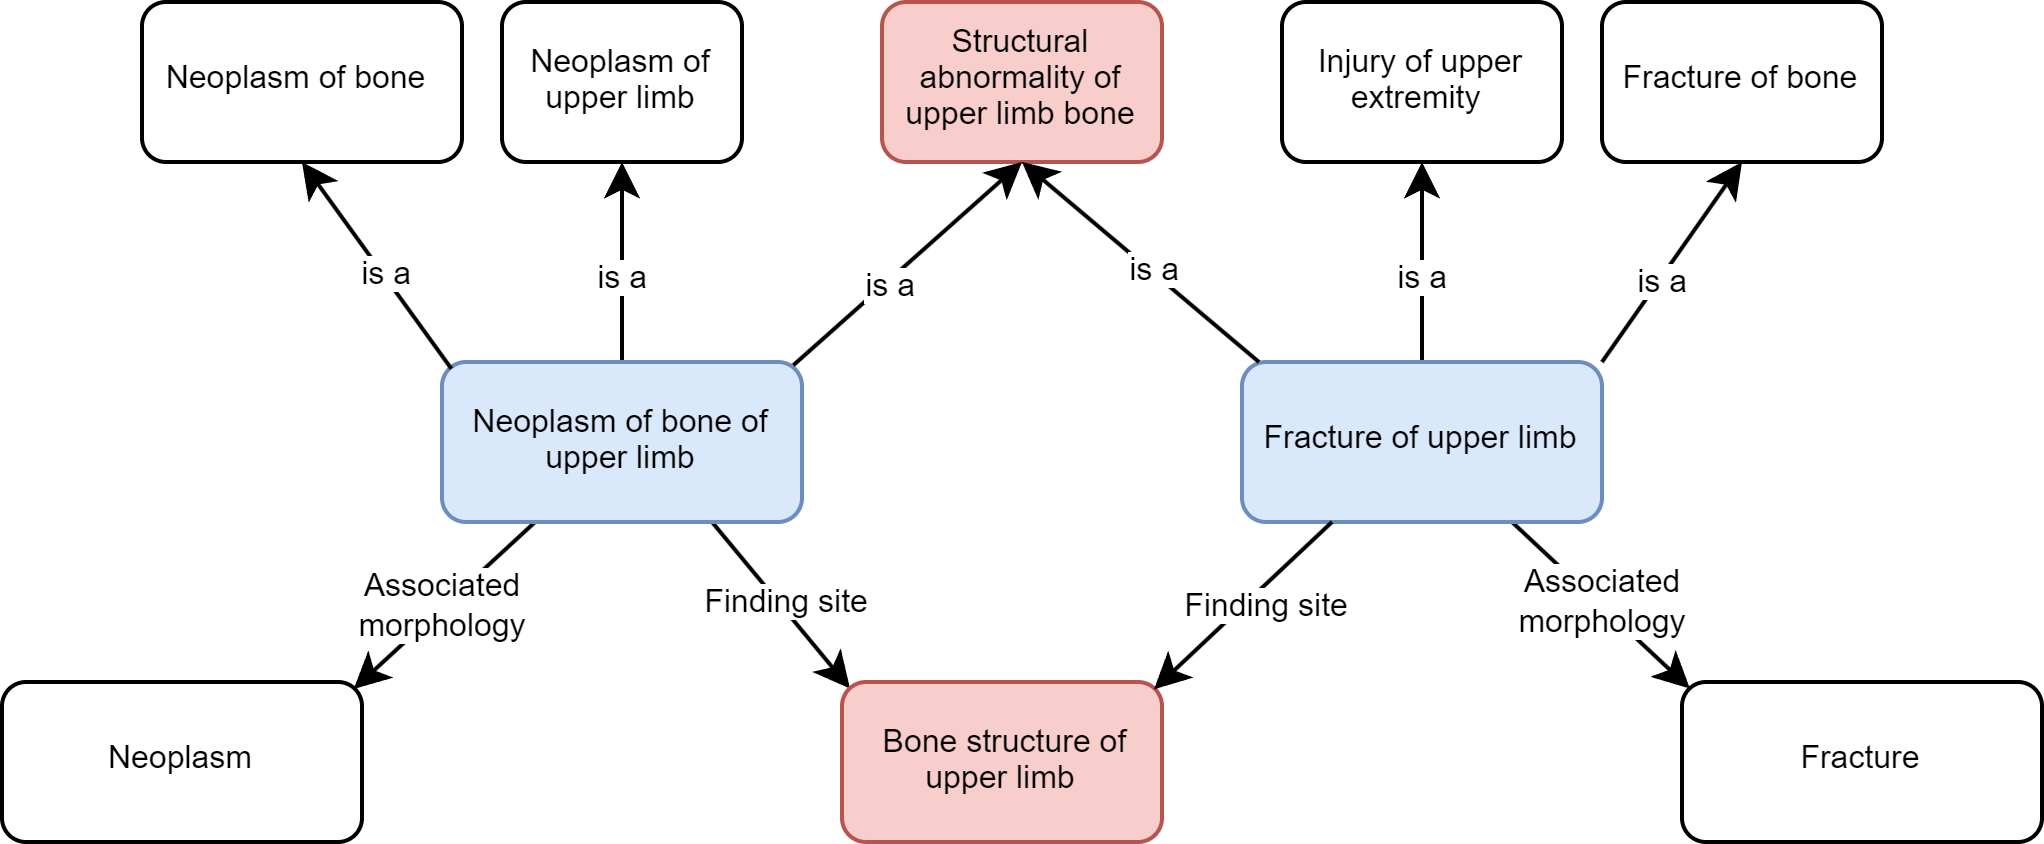
\includegraphics[width=\linewidth]{imgs/concept_relations.png}
\caption{Two SNOMED~CT disorders (blue) and their direct neighbours. Upward edges are \isa{} relationships to more general concepts; downward edges are attribute relationships, whose targets are values of the attribute rather than more general concepts. The two disorders differ, yet share a parent (\emph{Structural abnormality of upper limb bone}) and a finding site (\emph{Bone structure of upper limb}), shown in red.}
\label{fig:shared-structure}
\end{figure}

\section{Method}
\label{sec:method}

Our goal is to represent the concepts of an ontology with a small vocabulary of the ontology's own concepts, while preserving as much of their meaning as possible.
Section~\ref{sec:method:problem} states the problem.
Sections~\ref{sec:method:candidates}--\ref{sec:method:selection} select the vocabulary, Section~\ref{sec:method:tokenizer} writes each concept with it, and Section~\ref{sec:method:metrics} measures how much meaning is preserved.
Sections~\ref{sec:method:baselines}--\ref{sec:method:expert} describe the three experiments: a benchmark against graph baselines, an application to real EHR data, and an expert evaluation.

% ------------------------------------------------------------------
\subsection{Problem statement}
\label{sec:method:problem}

We model the ontology as a directed acyclic graph (DAG) $G = (V, E)$ with typed edges, $E \subseteq V \times \mathcal{R} \times V$.
An edge $(u, R, v)$ states that $v$ is a parent of $u$ ($R = \isa$) or the value of one of its attributes ($R \neq \isa$; Section~\ref{sec:snomed}).
Edges therefore point from a concept to the concepts that describe it, and acyclicity guarantees that following them never leads back to the starting concept.
The hop distance $d(u, v)$ is the number of edges on a shortest directed path from $u$ to $v$, over all relationship types.

Let $M \subseteq V$ be the concepts to represent; in our case, the concepts to which the codes of the clinical data are mapped.
Given a token budget $k$, we look for a token set $T \subseteq V$ of $k$ concepts such that every concept in $M$ can be described by the tokens it reaches, with as little loss of meaning as possible.
Because tokens are concepts of the ontology itself, every token has a known meaning that a domain expert can read.
Appendix~\ref{app:notation} lists the notation.

% ------------------------------------------------------------------
\subsection{Candidate pool}
\label{sec:method:candidates}

A concept can only be described by the concepts it reaches along the edges, and its meaning fades with each hop.
We therefore draw tokens from the concepts within $D$ hops of $M$:
\[
V_D = M \cup \{\, u \in V \setminus \{r\} : d(m, u) \le D \text{ for some } m \in M \,\},
\]
where $r$ is the root concept, which every concept reaches and which carries no meaning.
We write $G_D = (V_D, E_D)$ for the subgraph induced by $V_D$.
A larger hop radius $D$ admits more general candidates at a higher computational cost; Section~\ref{sec:setup} reports the value we use.

% ------------------------------------------------------------------
\subsection{Semantic coverage with distance decay}
\label{sec:method:score}

To select tokens, we need a score of how well a token set $T$ preserves the meaning of a concept.
Let $\mathrm{Out}(u)$ be the outgoing edges of $u$ in $G_D$ and $\deg^+(u) = |\mathrm{Out}(u)|$ its out-degree.
We define the \emph{semantic coverage} $S_h(u, T) \in [0, 1]$ of a concept $u$ recursively over the horizon $h \in \{0, \dots, D\}$, the number of hops still allowed.
At horizon~0, a concept is covered only if it is a token, $S_0(u, T) = \mathbf{1}[u \in T]$, and for $h \ge 1$,
\begin{equation}
S_h(u, T) =
\begin{cases}
1, & u \in T, \\[2pt]
0, & u \notin T \text{ and } \deg^+(u) = 0, \\[2pt]
\dfrac{\lambda}{\deg^+(u)} \displaystyle\sum_{(u,R,v) \in \mathrm{Out}(u)} S_{h-1}(v, T), & \text{otherwise,}
\end{cases}
\label{eq:coverage}
\end{equation}
where $\lambda \in [0, 1]$ is the \emph{distance decay}.
A token is fully covered, a concept that is not a token and has no outgoing edge is not covered, and any other concept takes the average coverage of its out-neighbours, multiplied by $\lambda$ for the hop.

Equivalently, $S_D(m, T)$ is the expected value of $\lambda^j$ over random walks that start at $m$ and follow a uniformly chosen outgoing edge at each step, where $j$ is the step at which the walk first meets a token (the value is 0 if it meets none within $D$ steps; Appendix~\ref{app:submodular}).
Each walk follows one strand of the concept's definition, and each hop replaces the current concept by a more general one or by one of its attribute values, so part of the meaning is lost at every hop.
With $\lambda = 1$, a walk counts fully as soon as it reaches a token, however far away; with $\lambda < 1$, near tokens count more than distant ones; with $\lambda = 0$, only concepts that are themselves tokens are covered.

The selection objective is the mean coverage of the concepts to represent,
\[
F_D(T) = \frac{1}{|M|} \sum_{m \in M} S_D(m, T).
\]
$F_D$ is normalized ($F_D(\varnothing) = 0$), monotone (adding a token never lowers it) and submodular (the gain from adding a token never grows as more tokens are selected); Appendix~\ref{app:submodular} gives the proof.

\paragraph{Status-dependent decay.}
The decay need not be the same for every hop.
In SNOMED~CT, a fully defined concept is equivalent to the conjunction of its relationships, whereas the relationships of a primitive concept are necessary but not sufficient to define it (Section~\ref{sec:snomed}).
A hop into a fully defined concept therefore rewrites the meaning without losing any of it, whereas a hop into a primitive concept is where meaning can be lost.
This is expressed by replacing $\lambda$ in Eq.~\eqref{eq:coverage} with a factor that depends on the target of the hop:
\begin{equation}
S_h(u, T) = \frac{1}{\deg^+(u)} \sum_{(u,R,v) \in \mathrm{Out}(u)} \lambda(v)\, S_{h-1}(v, T),
\qquad
\lambda(v) =
\begin{cases}
1, & v \text{ fully defined},\\
\lambda, & v \text{ primitive}.
\end{cases}
\label{eq:coverage-status}
\end{equation}
A walk then contributes the product of the factors of its hops up to its first token.
Since every factor lies in $[0, 1]$, the proof of Appendix~\ref{app:submodular} holds unchanged, and so do the selection algorithm and its guarantee (Section~\ref{sec:method:selection}).
The same holds for any factor in $[0, 1]$ attached to an edge, for instance one that depends on the relationship type.
In this paper, we use the uniform decay of Eq.~\eqref{eq:coverage}, which needs no concept status and applies to any DAG ontology.

% ------------------------------------------------------------------
\subsection{Lazy greedy token selection}
\label{sec:method:selection}

Greedy selection builds $T$ one token at a time, adding at each step the candidate $t \in V_D \setminus T$ with the largest marginal gain $\Delta(t \mid T) = F_D(T \cup \{t\}) - F_D(T)$.
Because $F_D$ is monotone and submodular, the greedy set $T_k$ is within a factor $1 - 1/e$ of the best set of the same size \cite{nemhauser1978analysis}:
\begin{equation}
F_D(T_k) \ge \Big(1 - \tfrac{1}{e}\Big) \max_{T \subseteq V_D,\ |T| \le k} F_D(T).
\label{eq:guarantee}
\end{equation}
The guarantee concerns the objective $F_D$ only; the context trees and the metrics of Section~\ref{sec:method:metrics} are computed separately, and the guarantee does not extend to them.
Submodularity also allows lazy evaluation \cite{minoux1978accelerated}.
A gain computed earlier is an upper bound on the current gain of the same candidate, so at each step only the candidate with the highest bound is re-evaluated: it is selected if its updated gain is still the highest, and is put back with its updated gain otherwise.
Lazy greedy returns the same tokens as plain greedy without re-evaluating every candidate at every step.

Each gain is computed incrementally.
Adding $t$ changes the coverage only of the concepts that reach $t$ within $D$ hops, so the change is propagated backward from $t$ along incoming edges, one hop per round, and touches only this reverse neighbourhood $R_D(t)$.
One evaluation costs $O(D \cdot |E(R_D(t))|)$, where $E(R_D(t))$ are the edges among the concepts of $R_D(t)$, instead of $O(D(|V_D| + |E_D|))$ for a full recomputation; in a sparse graph such as SNOMED~CT, $R_D(t)$ is usually small.
Appendix~\ref{app:algorithms} gives the algorithms.

Finally, greedy selection never removes a token, so the token set for any budget is a prefix of the same ranking: one run gives the vocabulary for every budget $k$.

% ------------------------------------------------------------------
\subsection{Context trees}
\label{sec:method:tokenizer}

Once $T$ is fixed, each concept of $M$ must be written with tokens.
The simplest representation is the flat set of tokens that a concept reaches, but this set loses which relationship led to which token.
In Figure~\ref{fig:context-tree}a, a disorder has two finding sites, the left kidney and the right adrenal gland.
Its flat set $\{\textit{kidney}, \textit{adrenal gland}, \textit{left}, \textit{right}\}$ cannot tell it apart from a disorder of the right kidney and the left adrenal gland.
The same loss occurs whenever a token is reached through a chain of attributes, as for the laterality of any paired body structure.

We therefore represent each concept by a \emph{context tree}, built by a forward traversal from the concept, bounded by $D$, with three rules:
\begin{itemize}
    \item \isa{} edges are \emph{transparent}: a parent describes the same aspect of the concept at a more general level, so the search continues in the current context;
    \item every other edge $(u, R, v)$ opens a \emph{subcontext} keyed by $(R, v)$, since it introduces a new aspect of the definition;
    \item each branch stops at its first token, which is attached to the current context together with its \emph{depth}, the number of hops from the concept; a branch that reaches depth $D$, or a concept without outgoing edges, without meeting a token is marked \emph{uncovered}.
\end{itemize}
In Figure~\ref{fig:context-tree}a, each finding site opens its own subcontext, so \textit{left} stays with \textit{kidney} and \textit{right} with \textit{adrenal gland}.

Algorithm~\ref{alg:expand} implements these rules; it is called once per concept as \textsc{Expand}$(m, q_0, 0)$, with an empty initial context $q_0$.
Two details matter.
The token test comes before the depth test, so a token at depth $D$ is accepted, as in Eq.~\eqref{eq:coverage}.
Attribute edges are expanded before \isa{} edges, and a pair $(R, v)$ already present in the current context is not expanded again: SNOMED~CT concepts often restate the attributes of their parents, and this rule keeps one subcontext per attribute, at the level of the child.
Figure~\ref{fig:context-tree}b traces the algorithm on a toy graph; the resulting tree, written as a nested expression, is $\big(t_A,\ R_1(t_B,\ R_2(\varnothing))\big)$, where $\varnothing$ marks an uncovered branch.

\begin{figure}[t]
\centering
\begin{minipage}[c]{0.04\linewidth}\small (a)\end{minipage}%
\begin{minipage}[c]{0.54\linewidth}
\centering
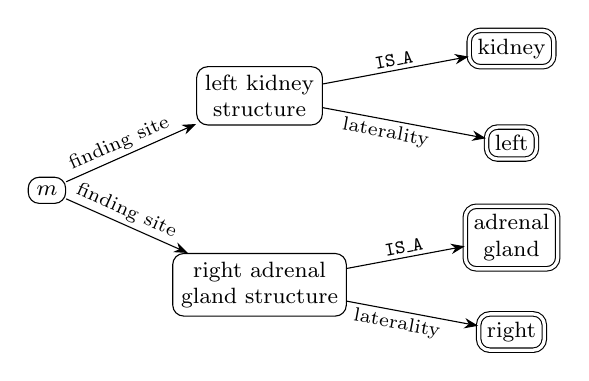
\begin{tikzpicture}[
  concept/.style={draw, rounded corners, align=center, font=\footnotesize, inner sep=3pt},
  token/.style={concept, double, double distance=1.2pt},
  rel/.style={-{Stealth[length=5pt]}},
  lab/.style={font=\scriptsize, inner sep=1.5pt}
]
\node[concept] (m) at (0,0) {$m$};
\node[concept] (lk) at (2.7,1.2) {left kidney\\structure};
\node[concept] (ra) at (2.7,-1.2) {right adrenal\\gland structure};
\node[token] (k) at (5.9,1.8) {kidney};
\node[token] (l) at (5.9,0.6) {left};
\node[token] (ag) at (5.9,-0.6) {adrenal\\gland};
\node[token] (r) at (5.9,-1.8) {right};
\draw[rel] (m) -- node[lab, sloped, above, pos=0.45] {finding site} (lk);
\draw[rel] (m) -- node[lab, sloped, above, pos=0.45] {finding site} (ra);
\draw[rel] (lk) -- node[lab, sloped, above] {\texttt{IS\_A}} (k);
\draw[rel] (lk) -- node[lab, sloped, below, pos=0.4] {laterality} (l);
\draw[rel] (ra) -- node[lab, sloped, above] {\texttt{IS\_A}} (ag);
\draw[rel] (ra) -- node[lab, sloped, below, pos=0.4] {laterality} (r);
\end{tikzpicture}
\end{minipage}\hfill
\begin{minipage}[c]{0.38\linewidth}
\begin{forest}
  for tree={font=\footnotesize, grow'=0, folder, folder indent=0.6em, inner sep=1.5pt},
  tok/.style={draw, double, double distance=1pt, rounded corners=2pt}
  [{$q_0$}
    [{finding site $[q_1]$}
      [kidney, tok]
      [{laterality $[q_2]$}
        [left, tok]]]
    [{finding site $[q_3]$}
      [{adrenal gland}, tok]
      [{laterality $[q_4]$}
        [right, tok]]]]
\end{forest}
\end{minipage}

\vspace{1.2em}
\begin{minipage}[c]{0.04\linewidth}\small (b)\end{minipage}%
\begin{minipage}[c]{0.54\linewidth}
\centering
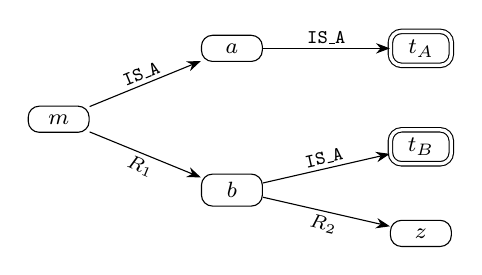
\begin{tikzpicture}[
  concept/.style={draw, rounded corners, align=center, font=\footnotesize, inner sep=3pt, minimum width=2.2em},
  token/.style={concept, double, double distance=1.2pt},
  rel/.style={-{Stealth[length=5pt]}},
  lab/.style={font=\scriptsize, inner sep=1.5pt}
]
\node[concept] (m) at (0,0) {$m$};
\node[concept] (a) at (2.2,0.9) {$a$};
\node[concept] (b) at (2.2,-0.9) {$b$};
\node[token] (tA) at (4.6,0.9) {$t_A$};
\node[token] (tB) at (4.6,-0.35) {$t_B$};
\node[concept] (z) at (4.6,-1.45) {$z$};
\draw[rel] (m) -- node[lab, sloped, above] {\texttt{IS\_A}} (a);
\draw[rel] (m) -- node[lab, sloped, below] {$R_1$} (b);
\draw[rel] (a) -- node[lab, above] {\texttt{IS\_A}} (tA);
\draw[rel] (b) -- node[lab, sloped, above] {\texttt{IS\_A}} (tB);
\draw[rel] (b) -- node[lab, sloped, below] {$R_2$} (z);
\end{tikzpicture}
\end{minipage}\hfill
\begin{minipage}[c]{0.38\linewidth}
\begin{forest}
  for tree={font=\footnotesize, grow'=0, folder, folder indent=0.6em, inner sep=1.5pt},
  tok/.style={draw, double, double distance=1pt, rounded corners=2pt}
  [{$q_0$}
    [{$t_A$}, tok]
    [{$R_1$ $[q_1]$}
      [{$t_B$}, tok]
      [{$R_2$ $[q_2]$}
        [{uncovered ($\varnothing$)}]]]]
\end{forest}
\end{minipage}
\caption{Context trees. Left: the graph around a concept $m$; double-bordered concepts are tokens. Right: the context tree of $m$.
(a)~Why trees are needed: each \emph{finding site} edge opens its own subcontext, so \textit{left} stays with \textit{kidney} and \textit{right} with \textit{adrenal gland}; the flat set $\{\textit{kidney}, \textit{adrenal gland}, \textit{left}, \textit{right}\}$ loses this pairing.
(b)~\textsc{Expand} on a toy graph with $D = 2$ and $T = \{t_A, t_B\}$: \isa{} keeps $t_A$ in the initial context $q_0$, $R_1$ opens $q_1$, which holds $t_B$, and $R_2$ opens $q_2$, whose branch reaches depth $D$ at the non-token $z$ and is uncovered.}
\label{fig:context-tree}
\end{figure}

\begin{algorithm}[t]
\caption{\textsc{Expand}$(u, q, \ell)$: builds the context tree of a concept $m$, called as \textsc{Expand}$(m, q_0, 0)$; $\ell$ counts the hops from $m$.}
\label{alg:expand}
\begin{algorithmic}[1]
\Procedure{Expand}{$u, q, \ell$}
    \If{$u \in T$} \Comment{token test first: a token at depth $D$ is accepted}
        \State attach $u$ as a token of context $q$ at depth $\ell$
        \State \Return
    \EndIf
    \If{$\ell = D$ \textbf{or} $\mathrm{Out}(u) = \varnothing$}
        \State mark this branch of $q$ as uncovered
        \State \Return
    \EndIf
    \ForAll{$(u, R, v) \in \mathrm{Out}(u)$, attribute edges before \texttt{IS\_A} edges}
        \If{$R = \texttt{IS\_A}$}
            \State \Call{Expand}{$v, q, \ell + 1$} \Comment{transparent: same context}
        \ElsIf{$q$ has no subcontext keyed by $(R, v)$}
            \State create subcontext $q'$ of $q$ keyed by $(R, v)$
            \State \Call{Expand}{$v, q', \ell + 1$}
        \EndIf
    \EndFor
\EndProcedure
\end{algorithmic}
\end{algorithm}

% ------------------------------------------------------------------
\subsection{Evaluating a tokenization}
\label{sec:method:metrics}

A tokenizer must meet four requirements at once: represent every concept, keep its meaning, keep concepts apart, and do so with short representations.
These requirements pull against each other under a fixed budget, so no single number captures the quality of a tokenization.
We therefore evaluate every token set with four core metrics, one per requirement (Table~\ref{tab:metrics}), and compare methods on all four jointly (Section~\ref{sec:results:benchmark}).

For a concept $m$, let $n_m$ be the number of tokens in its context tree, counting a token each time it appears, and $u_m$ the number of uncovered branches.
The \emph{signature} $\sigma_m$ of the tree is its nested structure of relationships, tokens and uncovered branches, without depths or order; we write $N_s$ for the number of concepts of $M$ whose signature is $s$.
The core metrics are computed per concept and averaged over $M$.

\paragraph{Represent every concept: unknown rate.}
The unknown rate is the share of concepts without any token ($n_m = 0$).
Like out-of-vocabulary words, these concepts lose all their information, so a tokenizer should leave none.

\paragraph{Keep the meaning: proximity-coverage score.}
A represented concept still loses meaning in two ways: whole branches of its definition are lost when no token is found, and specificity is lost when the tokens found are far away.
The \emph{proximity-coverage} (PC) score combines both.
It explores the same paths as Algorithm~\ref{alg:expand}, with the same stopping rules but without merging repeated subcontexts, and weights each branch by its share of the definition: a concept splits its weight equally among its outgoing relationships.
For a concept $u$ reached after $\ell$ hops,
\begin{equation}
\phi(u, \ell) =
\begin{cases}
1 - \dfrac{\ell}{D + 1}, & u \in T, \\[4pt]
0, & u \notin T \text{ and } (\ell = D \text{ or } \deg^+(u) = 0), \\[4pt]
\dfrac{1}{\deg^+(u)} \displaystyle\sum_{(u,R,w) \in \mathrm{Out}(u)} \phi(w, \ell + 1), & \text{otherwise,}
\end{cases}
\quad
\mathrm{PC}_m = \phi(m, 0).
\label{eq:pc}
\end{equation}
Unrolling the recursion, each branch $b$ of the expansion, a path from $m$ to its first token or to an uncovered end, receives a weight $\omega_b$, the product of $1/\deg^+(u)$ over the concepts $u$ it leaves; these weights sum to 1.
With $B^{+}_m$ the branches that end at a token, at depth $\ell_b$,
\[
\mathrm{PC}_m = c_m \cdot p_m,
\qquad
c_m = \sum_{b \in B^{+}_m} \omega_b,
\qquad
p_m = \frac{1}{c_m} \sum_{b \in B^{+}_m} \omega_b \Big(1 - \frac{\ell_b}{D + 1}\Big).
\]
The \emph{branch coverage} $c_m$ is the weight of the branches that end at a token, and the \emph{proximity} $p_m$ is their weighted mean closeness.
$\mathrm{PC}_m$ equals 1 when the concept is itself a token and 0 when it reaches no token.
In Figure~\ref{fig:context-tree}b, $m$ gives half of its weight to $a$, whose branch ends at $t_A$, and half to $b$, which splits it between $t_B$ and the uncovered $z$; both tokens lie at depth 2, so $c_m = 3/4$, $p_m = 1/3$ and $\mathrm{PC}_m = 1/4$.

The weights matter when the branches of a concept fan out unevenly.
Take a concept with two relationships, one leading to ten tokens at depth 2 and the other ending without a token ($D = 9$).
An unweighted mean over its eleven branch ends gives 0.73, more than the 0.45 the concept gets when the first relationship is itself a token at depth 1, although one closer token is the better representation: the many tokens of one branch hide the missing one.
With the weights, each relationship keeps half of the score, which gives 0.40 and 0.45.
In terms of random walks, $\mathrm{PC}_m$ is the expected value of $1 - j/(D + 1)$ over the walks of Section~\ref{sec:method:score}, where $j$ is the step of the first token (0 if none), and $c_m$ equals $S_D(m, T)$ at $\lambda = 1$.
The PC score thus uses the same walks as the selection objective, with a linear rather than geometric discount, and is not independent of it.
We therefore also report the unweighted mean (Appendix~\ref{app:flat-pc}), which ranks the methods in the same way, and compare the trees with expert judgement (Section~\ref{sec:method:expert}).

\paragraph{Keep concepts apart: unique rate.}
The unique rate is the share of concepts whose signature no other concept has ($N_{\sigma_m} = 1$).
Two concepts with the same tree are indistinguishable for a model, however well each of them is covered.

\paragraph{Stay short: tokens per concept.}
The number of tokens per concept, the mean of $n_m$, measures the efficiency of the tokenizer.
It sets the length of the input sequences, and the cost of standard self-attention grows quadratically with this length \cite{vaswani2017attention}.
On EHR data, we report the corresponding cost per event (Section~\ref{sec:method:ehr}).

The four metrics cannot be optimized one at a time.
A vocabulary of generic hub concepts reaches every concept, but through long and distant branches, which lowers the PC score and lengthens the trees.
A vocabulary of very specific concepts keeps the trees short and close for the concepts it contains, but leaves others unknown.
Two concepts can both score high on PC and still share one tree.
We therefore compare methods by their average rank over the four metrics rather than on any one of them.
As secondary metrics, the \emph{uncovered branch rate} is the share of concepts with at least one uncovered branch ($u_m > 0$), which keep only part of their definition, and the \emph{vocabulary use} is the share of the $k$ selected tokens that appear in at least one context tree.
A token that no concept uses takes a slot of the vocabulary, and an embedding, without serving any concept.
Because a mean can hide a minority of badly represented concepts, we also report the distribution of the per-concept PC score and number of tokens.
\begin{table}[t]
\centering
\small
\renewcommand{\arraystretch}{1.3}
\setlength{\tabcolsep}{4pt}
\begin{tabular}{@{}llcc@{}}
\toprule
\textbf{Requirement} & \textbf{Metric} & \textbf{Per concept} & \textbf{Better} \\
\midrule
Represent every concept & Unknown rate & $\mathbf{1}[n_m = 0]$ & $\downarrow$ \\
Keep its meaning & Proximity-coverage (PC) score & $c_m \cdot p_m$, Eq.~\eqref{eq:pc} & $\uparrow$ \\
Keep concepts apart & Unique rate & $\mathbf{1}[N_{\sigma_m} = 1]$ & $\uparrow$ \\
Stay short (efficiency) & Tokens per concept & $n_m$ & $\downarrow$ \\
\midrule
Keep the whole definition (secondary) & Uncovered branch rate & $\mathbf{1}[u_m > 0]$ & $\downarrow$ \\
Use the whole vocabulary (secondary) & Vocabulary use & -- (per token set) & $\uparrow$ \\
\bottomrule
\end{tabular}
\caption{Evaluation metrics: one core metric per requirement of a tokenizer. The per-concept metrics are averaged over the concepts to represent; vocabulary use is the share of the $k$ tokens that at least one context tree contains.}
\label{tab:metrics}
\end{table}

% ------------------------------------------------------------------
\subsection{Compared selection methods}
\label{sec:method:baselines}

We compare 19 configurations (Table~\ref{tab:baselines}), which all select their tokens from the same candidate pool $V_D$.
Except for random selection, each configuration ranks $V_D$ once and takes the top $k$ candidates, so one ranking serves every budget.

\paragraph{Our method.} We run our selection with $\lambda \in \{0, 0.1, \dots, 1\}$.

\paragraph{Ablation: discrete set cover.}
The ablation uses the same lazy greedy procedure and has the same guarantee, but replaces $S_h(u, T)$ by a binary indicator: a concept counts as covered as soon as some token lies within $D$ hops of it, however far away and through however few of its branches.
This is the classical maximum coverage problem \cite{nemhauser1978analysis, feige1998threshold}.
Since the procedure is identical, the difference between the two isolates the effect of the distance-aware coverage.

\paragraph{Baselines.}
Seven baselines are well defined on a DAG: random selection, three degree-based rankings and three centrality-based rankings (Table~\ref{tab:baselines}).
Degree- and PageRank-based selection also correspond to the anchor-selection strategies of NodePiece~\cite{galkin2022nodepiece}.

\begin{table}[t]
\centering
\small
\renewcommand{\arraystretch}{1.2}
\setlength{\tabcolsep}{4pt}
\begin{tabular}{@{}>{\raggedright\arraybackslash}p{1.6cm}>{\raggedright\arraybackslash}p{3.0cm}c>{\raggedright\arraybackslash}p{7.6cm}@{}}
\toprule
\textbf{Family} & \textbf{Method} & \textbf{Configs} & \textbf{Ranks candidates by} \\
\midrule
Ours & Semantic coverage greedy & 11 & marginal gain in $F_D$, $\lambda \in \{0, 0.1, \dots, 1\}$ \\
Ablation & Discrete set cover & 1 & marginal gain in the number of concepts with a token within $D$ hops \\
Random & Random & 1 & uniform sampling; metrics averaged over 20 draws \\
\midrule
\multirow{3}{*}{Degree} & Highest degree, $d \le D$ & 1 & number of concepts that reach the candidate within $D$ hops \\
 & Highest degree, $d \le 1$ & 1 & number of concepts that reach the candidate in one hop \\
 & Most \isa{} children & 1 & number of descendants within $D$ \isa{} hops \\
\midrule
\multirow{3}{*}{Centrality} & PageRank & 1 & stationary probability of a random walk restarting uniformly on $V_D$, $\alpha = 0.85$ \cite{page1999pagerank} \\
 & Personalized PageRank & 1 & same walk, restarting uniformly on $M$ \cite{haveliwala2002topic} \\
 & Closeness centrality & 1 & inverse mean distance from the concepts that reach the candidate, with the Wasserman--Faust correction \cite{freeman1978centrality, wasserman1994social} \\
\midrule
\multicolumn{2}{@{}l}{\textbf{Total}} & 19 & \\
\bottomrule
\end{tabular}
\caption{The 19 compared configurations. All select from the candidate pool $V_D$.}
\label{tab:baselines}
\end{table}

% ------------------------------------------------------------------
\subsection{Application to EHR data}
\label{sec:method:ehr}

The benchmark treats all concepts alike, whereas in EHR data a few concepts produce most events and most concepts are rare.
We therefore apply the tokenizer to the concepts $\Mhero$ that occur in a real EHR dataset (Section~\ref{sec:setup}).
We re-run the whole pipeline on $\Mhero$ (candidate pool, then selection with $\lambda = 0.9$); the selection uses only the list of concepts, not their frequencies.
An \emph{event} is one recorded occurrence of a concept.

We compare our tokenizer with \emph{frequency truncation}, the usual frequency-based reduction of EHR vocabularies \cite{steinberg2021language}: the $k$ most frequent concepts become tokens, and every other concept is mapped to a single unknown token.
We measure:
\begin{itemize}
    \item \emph{concepts and events represented}: a concept is represented if it receives at least one token other than the unknown token, and an event is represented if its concept is;
    \item \emph{rare concepts}: concepts with fewer than 100 events, for which we report the share represented and the PC score. For truncation, the PC score follows from its definition: a kept concept is its own token, at depth 0, and scores 1, and a discarded concept has no token and scores 0;
    \item \emph{borrowed strength}: a token occurs in every event of every concept that uses it, so a rare concept is learned from the events of its tokens rather than from its own; we compare the number of events of a concept with that of its least frequent token;
    \item \emph{tokens per event}: the length of the representation of an event, counting the distinct tokens of each context and one marker per subcontext; truncation always uses one token.
\end{itemize}

% ------------------------------------------------------------------
\subsection{Expert evaluation}
\label{sec:method:expert}

The PC score measures distance in the graph, not clinical meaning.
Semanticians therefore compared, blinded, the context trees of our tokenizer ($\lambda = 0.9$, $k = 5{,}000$, selected on $\Mhero$) with those of Personalized PageRank at the same budget, using the official SNOMED~CT definition of each concept as the reference.
We chose Personalized PageRank because it is the only baseline that, like our method, targets the concepts to represent: its random walk restarts on $M$. \doubt{state the rule fixed in advance; with the four-metric ranking, Personalized PageRank is the best baseline only at low compression}

\paragraph{Concepts.}
We consider the concepts of $\Mhero$ that belong to the official SNOMED~CT release, and keep those whose two trees differ; concepts with identical trees count as ``no clear difference''.
To keep the task feasible, the two trees of a concept may hold at most 16 tokens together.
Primitive concepts are included, since leaving them out would bias the sample; raters judge them by their name and stated relationships.
A concept falls into one of three categories: kept as a token by our method and decomposed by the baseline, the reverse, or decomposed by both into different trees.
We sampled 100 concepts, stratified by category and by definition status; every rater rates the same 100 concepts, in a rater-specific order, and the side (A or B) of each method is randomized and balanced within each stratum.

\paragraph{Task and analysis.}
For each concept, raters choose ``A better'', ``no clear difference'' or ``B better'', and may flag, for each version, an incorrect or ambiguous association, absent information, lost precision (too general a token), or redundant information.
For a fully defined concept, they may also flag an official definition that does not capture its meaning.
We report the preference among the rated concepts, per stratum and weighted by stratum size, with a sign test that excludes ties and bootstrap confidence intervals; separately, we report it over all concepts of the release, where concepts with identical trees count as ties.
We also report the agreement between raters (Cohen's $\kappa$, or Fleiss' $\kappa$ for more than two raters) and between expert preference and the sign of the difference in PC score.

\section{Results}
\label{sec:results}

We ask four questions about the meaning preserved by the tokenizer.
What does a tokenized concept look like (Section~\ref{sec:results:examples})?
Does our selection preserve meaning better than graph-based selections, and how do $k$ and $\lambda$ matter (Section~\ref{sec:results:benchmark})?
On real, long-tailed EHR data, are rare concepts preserved (Section~\ref{sec:results:hero})?
Do semanticians agree with the automatic metrics (Section~\ref{sec:results:expert})?

% ------------------------------------------------------------------
\subsection{Experimental setup}
\label{sec:setup}

We run two experiments with the same pipeline on two concept sets, each with its own candidate subgraph and candidate pool (Table~\ref{tab:setup}).
The benchmark uses no patient data; the EHR application uses real event counts.

\paragraph{Benchmark on the mapped concepts.}
The benchmark uses the set $M$ of 46,150 SNOMED~CT concepts to which the codes of the clinical data warehouse of the Geneva University Hospitals (HUG) were mapped by the institution's terminology experts \notetoself{SNOMED CT release used}.
It relies only on these concepts and on the ontology graph.
We set the hop radius to $D = 9$, which covers 98.4\% of the concept depths in the candidate subgraph.
The resulting subgraph $G_D$ is a DAG that keeps 103 of the 113 relationship types (Appendix~\ref{app:relations}).
Its 75,964 nodes form the candidate pool: the 46,150 mapped concepts and the 29,814 concepts they reach.
All 19 configurations of Section~\ref{sec:method:baselines} select their tokens from this pool, at the budgets $k = 500, 1{,}000, \dots, 19{,}500$, which we group into three compression levels of 13 budgets each (Table~\ref{tab:setup}b).

\paragraph{Application to real EHR data.}
The second experiment uses the structured patient data of the HERO project at HUG, collected between 2017 and 2025 \notetoself{ethics approval / general consent}, composed by 16,370 distinct SNOMED CT concepts and form the set $\Mhero$.
The concepts of $\Mhero$ occur in 279 million events from 937,096 patients.
We ran the whole pipeline again on $\Mhero$ alone, with the same hop radius $D = 9$, which gives a smaller candidate pool than in the benchmark (Table~\ref{tab:setup}a).
Token budgets are therefore not comparable between the two experiments: $k = 5{,}000$ is 10.8\% of $|M|$ but 30.5\% of $|\Mhero|$.
We evaluate budgets from $k = 250$ to $k = |\Mhero| = 16{,}370$ and compare our tokenizer with frequency truncation (Section~\ref{sec:method:ehr}).

\paragraph{Expert evaluation.}
Semanticians compared our tokenizer with Personalized PageRank at $k = 5{,}000$ on a stratified sample of 100 concepts of $\Mhero$, blinded, with the official SNOMED~CT definition as reference (Section~\ref{sec:method:expert}).

\begin{table}[t]
\centering
\small
\caption{Experimental setup. (a) Full SNOMED~CT graph $G$ and the two experiments, each with its own candidate subgraph ($D = 9$). (b) Compression levels of the benchmark; each level contains 13 token budgets in steps of 500.}
\label{tab:setup}
\begin{tabular}{@{}lrrr@{}}
\toprule
\multicolumn{4}{@{}l}{\textit{(a) Graphs and experiments}} \\
 & Full graph $G$ & Benchmark ($M$) & HERO ($\Mhero$) \\
\midrule
Concepts to represent & --        & 46,150      & 16,370 \\
Candidate pool (nodes)& 447,420   & 75,964      & 37,601 \\
Edges                 & 1,684,197 & 293,146     & 134,313 \\
Relationship types    & 113       & 103         & 87 \\
Token budgets $k$     & --        & 500--19,500 & 250--16,370 \\
Compared with         & --        & 18 other configurations & frequency truncation \\
\midrule
\multicolumn{4}{@{}l}{\textit{(b) Compression levels of the benchmark}} \\
Level & $k$ & $k/|M|$ (\%) & \\
\midrule
High & 500--6,500     & 1.1--14.1  & \\
Mid  & 7,000--13,000  & 15.2--28.2 & \\
Low  & 13,500--19,500 & 29.3--42.3 & \\
\bottomrule
\end{tabular}
\end{table}

% ------------------------------------------------------------------
\subsection{What a tokenized concept looks like}
\label{sec:results:examples}

Before comparing selection methods, we show what our tokenizer produces for three mapped concepts and how the metrics read on each of them (Figure~\ref{fig:example-trees}, Table~\ref{tab:example-trees}).
We fix $\lambda = 0.9$ and $k = 5{,}000$ ($k/|M| = 10.8\%$) for illustration only; Section~\ref{sec:results:benchmark} studies both parameters.
We chose concepts with shallow trees for readability.

\textit{Pain of breast} (Figure~\ref{fig:example-trees}a) has three outgoing relationships: a \textit{finding site} edge to \textit{breast structure}, and two \isa{} edges, to \textit{chest pain} and to \textit{finding of sensation of breast}.
Breast structure and chest pain are tokens at depth~1.
Finding of sensation of breast is not a token, so \textsc{Expand} continues through its two parents, \textit{finding of sensation by site} and \textit{breast finding}, which are tokens at depth~2.
Because \isa{} is transparent, these three tokens join the initial context, whereas the finding site opens a subcontext that holds breast structure.
Finding of sensation of breast has the same finding site as its child; since this pair is already in the initial context, it is not expanded again (dashed edge).
The resulting tree is
\[
\big(\textit{finding of sensation by site},\ \textit{breast finding},\ \textit{chest pain},\ \textit{finding site}(\textit{breast structure})\big).
\]
All its branches end at a token ($c_m = 1$), and its three relationships share the weight equally.
Breast structure and chest pain, at depth~1, contribute 0.9 each; finding of sensation of breast passes its third on to its own three relationships, including the restated finding site, which all end at tokens at depth~2 and contribute 0.8.
The concept therefore keeps most of its meaning, with $\mathrm{PC}_m = (0.9 + 0.9 + 0.8)/3 \approx 0.87$, and no other concept shares its tree.

\textit{Hyperthyroidism} and \textit{sick-euthyroid syndrome} (Figure~\ref{fig:example-trees}b) have the same two relationships: an \isa{} edge to \textit{disorder of thyroid gland} and a \textit{finding site} edge to \textit{thyroid structure}.
Both targets are tokens at depth~1, so both concepts receive the same tree,
\[
\big(\textit{disorder of thyroid gland},\ \textit{finding site}(\textit{thyroid structure})\big).
\]
Each tree scores well on its own ($\mathrm{PC}_m = 0.90$), yet a downstream model cannot tell the two concepts apart, although they describe different conditions: an overactive thyroid gland, and abnormal thyroid tests with a normal gland.
Both concepts are primitive: the graph does not state what distinguishes them, so no token set can separate them unless one of them becomes a token itself (Section~\ref{sec:limitations}).

\begin{figure}[t]
\centering
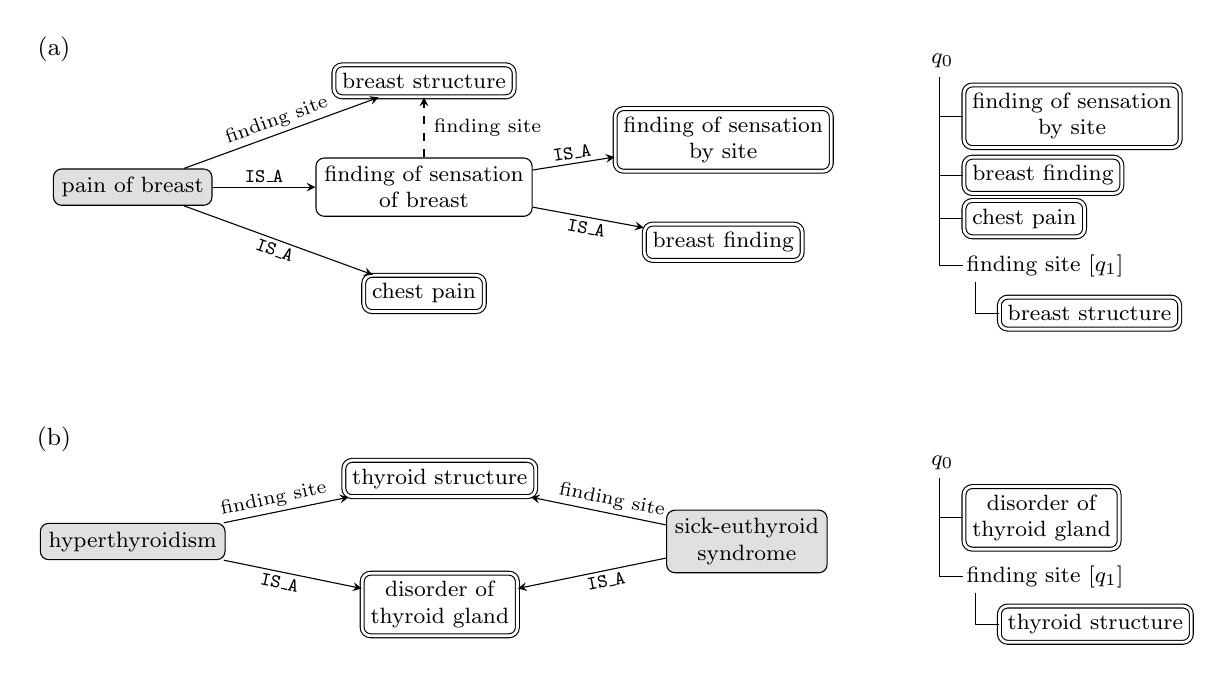
\begin{tikzpicture}[
  >=stealth,
  concept/.style={draw, rounded corners=3pt, align=center, font=\footnotesize, inner sep=3pt},
  mapped/.style={concept, fill=black!12},
  token/.style={concept, double, double distance=1pt},
  rel/.style={font=\scriptsize, sloped, above, inner sep=1.5pt},
  isa/.style={font=\scriptsize\ttfamily, sloped, above, inner sep=1.5pt},
  treeline/.style={draw, thin},
  ctx/.style={font=\footnotesize, anchor=west, inner sep=1pt},
]
% ---------------- (a) Pain of breast ----------------
\node[font=\small] at (-1.0, 1.75) {(a)};
\node[mapped] (pb) at (0,0) {pain of breast};
\node[token]   (bs)  at (3.7, 1.35) {breast structure};
\node[concept] (fsb) at (3.7, 0)    {finding of sensation\\ of breast};
\node[token]   (cp)  at (3.7,-1.35) {chest pain};
\node[token]   (fss) at (7.5, 0.6)  {finding of sensation\\ by site};
\node[token]   (bf)  at (7.5,-0.7)  {breast finding};
\draw[->] (pb) -- node[rel] {finding site} (bs);
\draw[->] (pb) -- node[isa] {IS\_A} (fsb);
\draw[->] (pb) -- node[isa,below] {IS\_A} (cp);
\draw[->] (fsb) -- node[isa] {IS\_A} (fss);
\draw[->] (fsb) -- node[isa,below] {IS\_A} (bf);
\draw[->,dashed] (fsb) -- node[font=\scriptsize, right] {finding site} (bs);
% context tree (a)
\begin{scope}[shift={(10.1,1.6)}]
  \node[ctx] at (0,0) {$q_0$};
  \node[token,anchor=west] (a1) at (0.45,-0.7)  {finding of sensation\\ by site};
  \node[token,anchor=west] (a2) at (0.45,-1.45) {breast finding};
  \node[token,anchor=west] (a3) at (0.45,-2.0)  {chest pain};
  \node[ctx]               (a4) at (0.45,-2.6)  {finding site [$q_1$]};
  \node[token,anchor=west] (a5) at (0.9,-3.2)   {breast structure};
  \foreach \n in {a1,a2,a3,a4} \draw[treeline] (0.15,-0.2) |- (\n.west);
  \draw[treeline] (0.6,-2.8) |- (a5.west);
\end{scope}
% ---------------- (b) Hyperthyroidism and sick-euthyroid syndrome ----------------
\begin{scope}[shift={(0,-4.5)}]
\node[font=\small] at (-1.0, 1.3) {(b)};
\node[mapped] (hy) at (0,0)    {hyperthyroidism};
\node[token]  (ts) at (3.9, 0.8) {thyroid structure};
\node[token]  (dt) at (3.9,-0.8) {disorder of\\ thyroid gland};
\node[mapped] (se) at (7.8,0)  {sick-euthyroid\\ syndrome};
\draw[->] (hy) -- node[rel, pos=0.42] {finding site} (ts);
\draw[->] (hy) -- node[isa, below, pos=0.42] {IS\_A} (dt);
\draw[->] (se) -- node[rel, pos=0.42] {finding site} (ts);
\draw[->] (se) -- node[isa, below, pos=0.42] {IS\_A} (dt);
% shared context tree (b)
\begin{scope}[shift={(10.1,1.0)}]
  \node[ctx] at (0,0) {$q_0$};
  \node[token,anchor=west] (b1) at (0.45,-0.7)  {disorder of\\ thyroid gland};
  \node[ctx]               (b2) at (0.45,-1.45) {finding site [$q_1$]};
  \node[token,anchor=west] (b3) at (0.9,-2.05)  {thyroid structure};
  \foreach \n in {b1,b2} \draw[treeline] (0.15,-0.2) |- (\n.west);
  \draw[treeline] (0.6,-1.65) |- (b3.west);
\end{scope}
\end{scope}
\end{tikzpicture}
\caption{Context trees of three mapped concepts at $\lambda = 0.9$ and $k = 5{,}000$. Left: the part of $G_D$ explored by \textsc{Expand}; mapped concepts are shaded and double-bordered concepts are tokens. Right: the resulting context tree. (a) \textit{Pain of breast} receives a unique tree; the dashed edge is a finding site that its parent restates, which is not expanded again. (b) \textit{Hyperthyroidism} and \textit{sick-euthyroid syndrome} reach the same two tokens through the same relationships, and therefore share one context tree.}
\label{fig:example-trees}
\end{figure}

\begin{table}[t]
\centering
\small
\caption{Per-concept values for the examples of Figure~\ref{fig:example-trees} ($\lambda = 0.9$, $k = 5{,}000$, $D = 9$). $n_m$: tokens; $u_m$: uncovered branches; PC: proximity-coverage score; $N_{\sigma_m}$: number of mapped concepts with the same tree.}
\label{tab:example-trees}
\begin{tabular}{@{}lllcclcc@{}}
\toprule
Concept & SCTID & Status & $n_m$ & $u_m$ & Token depths & PC & $N_{\sigma_m}$ \\
\midrule
Pain of breast          & 53430007  & fully defined & 4 & 0 & 1, 1, 2, 2 & 0.87 & 1 \\
Hyperthyroidism         & 34486009  & primitive     & 2 & 0 & 1, 1       & 0.90 & 2 \\
Sick-euthyroid syndrome & 237542005 & primitive     & 2 & 0 & 1, 1       & 0.90 & 2 \\
\bottomrule
\end{tabular}
\end{table}

% ------------------------------------------------------------------
\subsection{Comparison with graph-based selection, and effect of \texorpdfstring{$k$ and $\lambda$}{k and lambda}}
\label{sec:results:benchmark}

The examples show single concepts; we now evaluate the 19 configurations on all 46,150 mapped concepts.

\paragraph{Ranking.}
At each token budget, we rank the 19 configurations on each of the four core metrics, average the four ranks, and then average over the 13 budgets of each compression level (Appendix~\ref{app:ranking}).
No configuration wins every metric.
Our method with $\lambda = 0.9$ obtains the best average rank at every compression level, and every $\lambda$ from 0.5 to 0.9 outranks all baselines (Figure~\ref{fig:rank-by-family}).
The best baselines are highest degree ($d \le 1$) among the degree-based methods and Personalized PageRank among the centrality-based ones.
The set-cover ablation ranks below every $\lambda$ from 0.1 to 0.9 at every level, close to random selection.
Since it uses the same greedy procedure with a binary objective, the distance-aware objective, not greedy selection alone, drives the result.
The two extremes, $\lambda = 0$ and $\lambda = 1$, also rank near the bottom (Section~\ref{sec:discussion:why}).

\begin{figure*}[t]
\centering
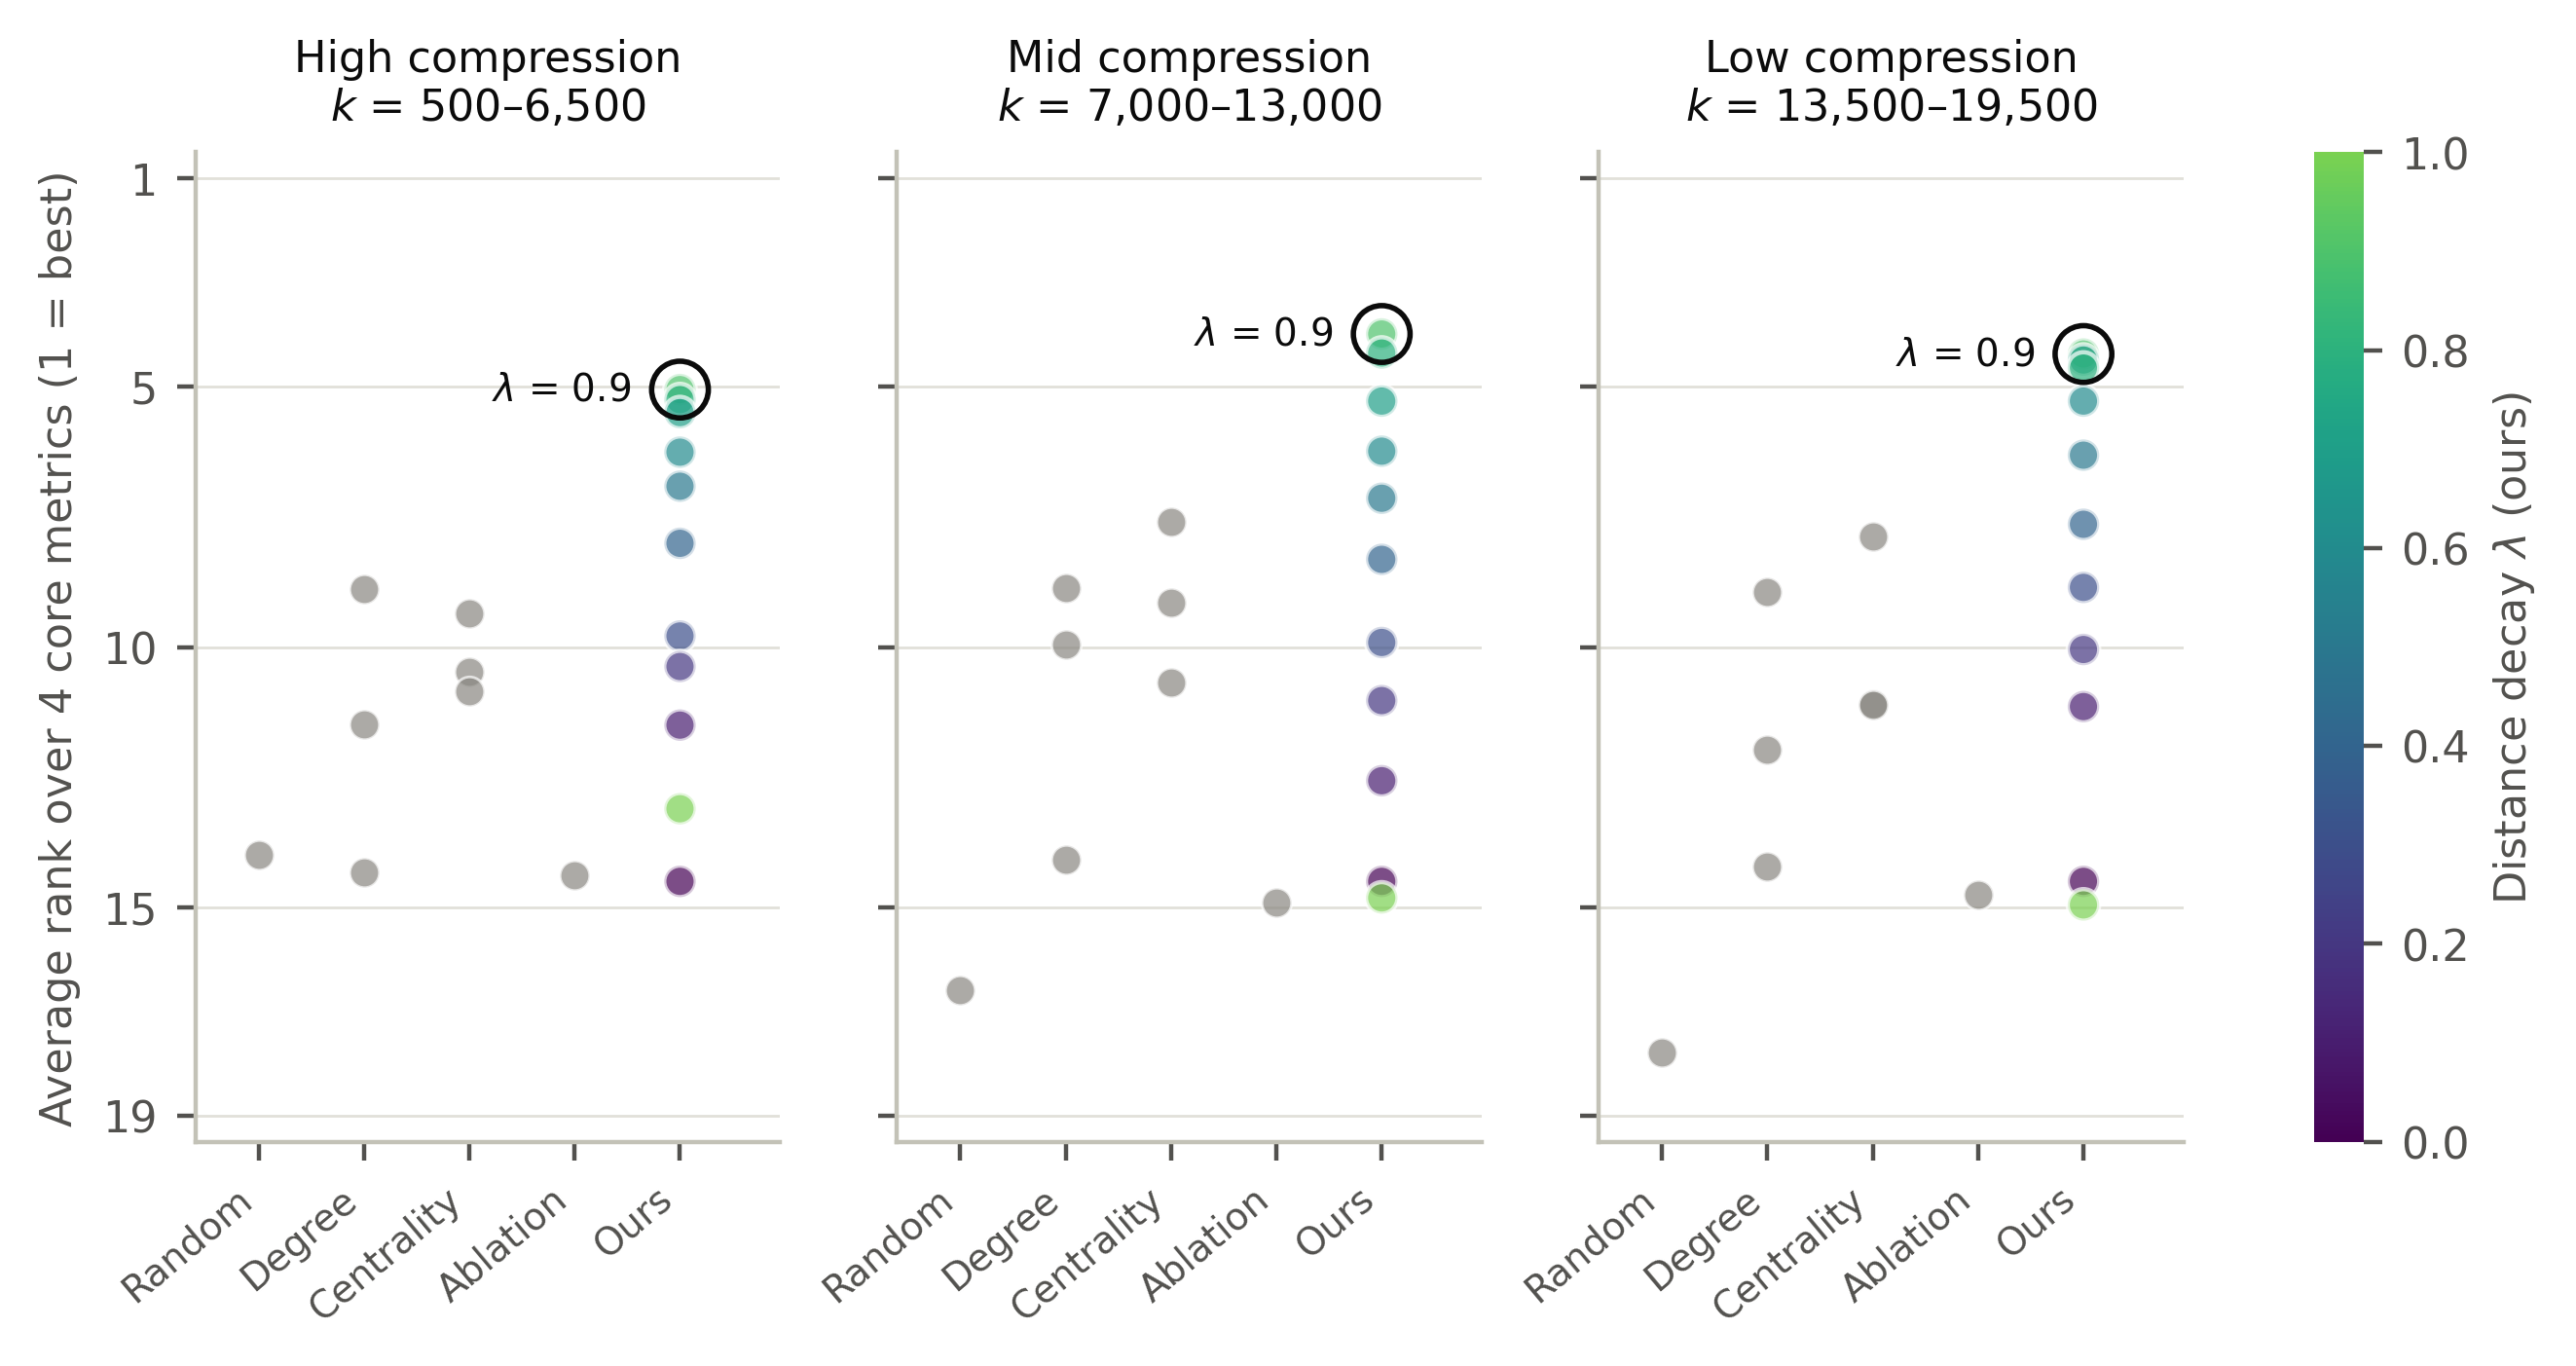
\includegraphics[width=\textwidth]{imgs/rank_by_family.png}
\caption{Average rank of the 19 configurations at each compression level (rank 1 = best), averaged over the four core metrics and the 13 token budgets per level. Gray points are baselines, with methods of the same family sharing a column; coloured points are our method at each value of the distance decay $\lambda$. The circled point marks the best configuration at each level ($\lambda = 0.9$ throughout).}
\label{fig:rank-by-family}
\end{figure*}

\paragraph{Effect of the token budget $k$.}
All methods follow the same trends (Figure~\ref{fig:metrics-vs-k}): the PC score and the unique rate increase with $k$, the number of tokens per concept decreases, and the unknown rate reaches zero early.
A larger vocabulary brings the nearest token closer to each concept, so branches stop earlier, which shortens the trees, and closer tokens are more specific, which separates more concepts.
Our method keeps a higher PC score than every baseline at every budget and leaves no concept without a token from $k = 1{,}000$ on, whereas highest degree ($d \le 1$) leaves unknown concepts up to $k = 13{,}500$.
The set-cover ablation has the lowest PC score and unique rate, and the longest trees, at every $k$.
The per-concept distributions show where the gain of a larger budget goes (Figure~\ref{fig:dist-k-lambda}).
For a typical concept, little changes: the median PC score rises only from 0.87 to 0.90, and the median number of tokens stays at four to five.
The gain goes to the worst-represented concepts: from high to low compression, the 10th percentile of the PC score rises from 0.79 to 0.87, and the 90th percentile of the number of tokens falls from 22 to 8.

\begin{figure*}[t]
\centering
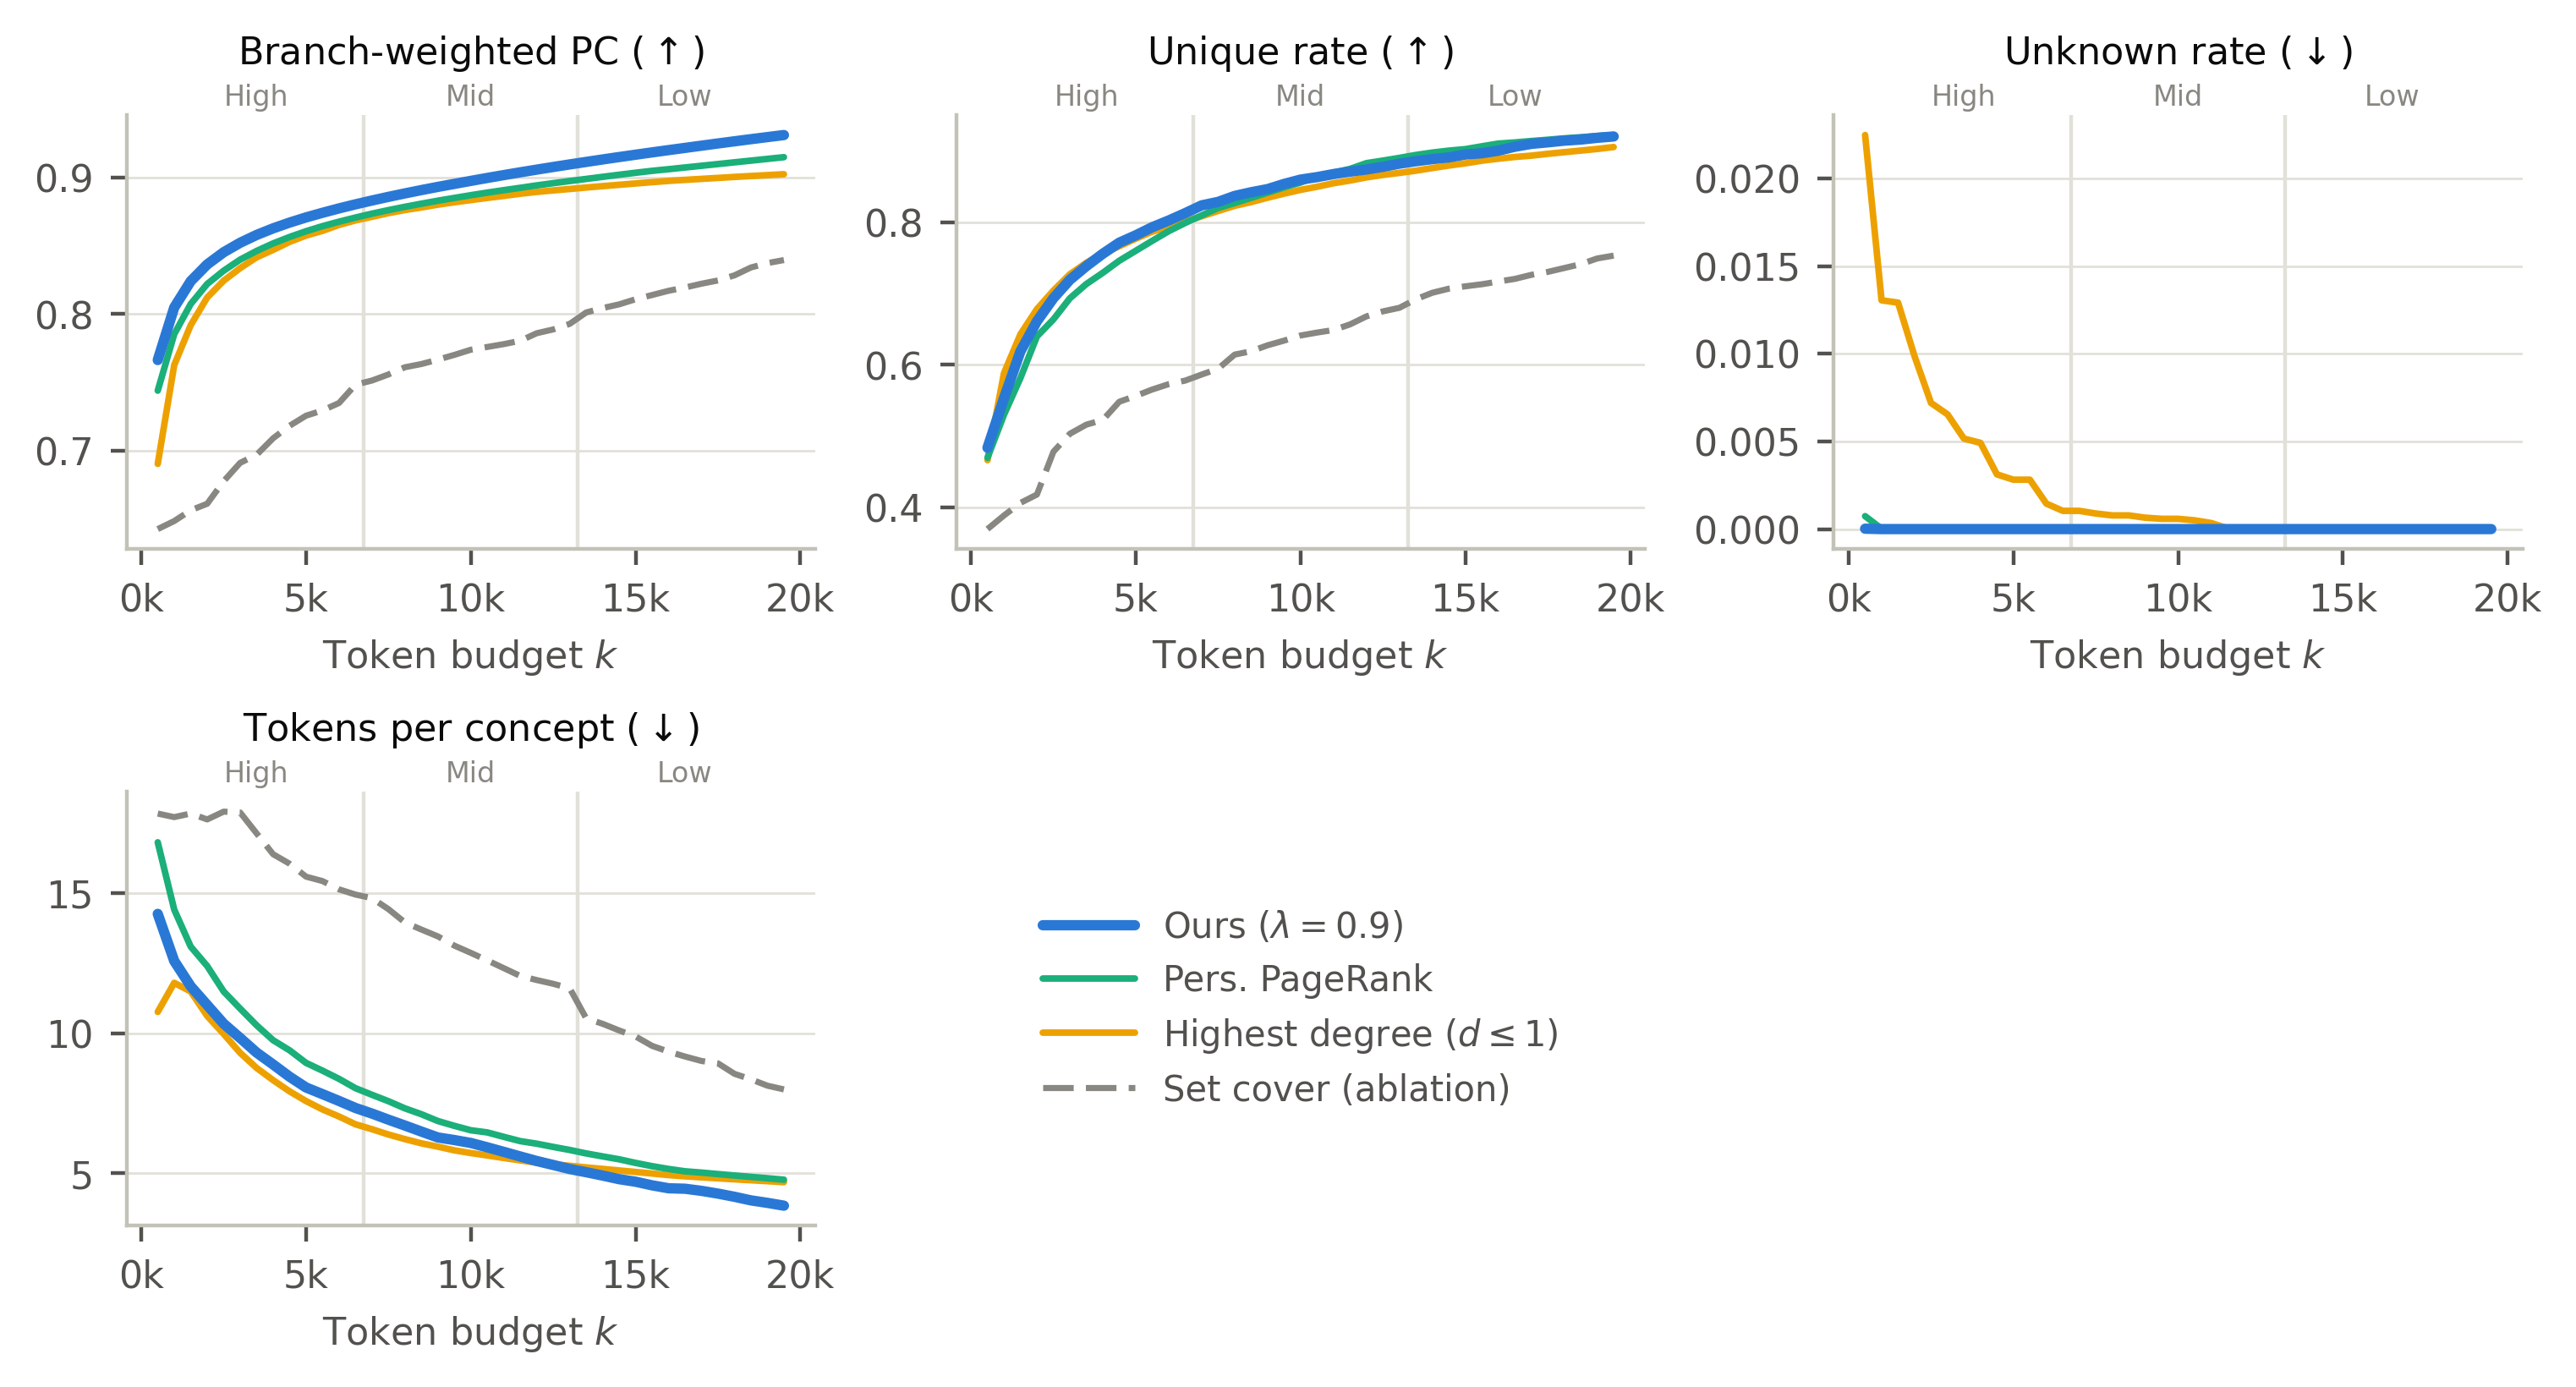
\includegraphics[width=\textwidth]{imgs/metrics_vs_k.png}
\caption{Core metrics as a function of the token budget $k$ for our method ($\lambda = 0.9$), the set-cover ablation, and the best baseline of each family (Personalized PageRank; highest degree, $d \le 1$).
Arrows indicate the preferred direction; vertical lines separate the high, mid and low compression levels (Table~\ref{tab:setup}b).
Random selection is in Appendix Figure~\ref{fig:metrics-vs-k-all}.}
\label{fig:metrics-vs-k}
\end{figure*}

\paragraph{Effect of the distance decay $\lambda$.}
Figure~\ref{fig:dist-k-lambda} compares three values of $\lambda$ between 0 and 1 with $\lambda = 1$, at one budget per compression level; Appendix~\ref{app:lambda} gives the mean metrics for every $\lambda$, including $\lambda = 0$.
From $\lambda = 0.3$ to $0.9$, the median PC score barely changes, but its lower tail rises: fewer concepts are left with only distant tokens.
The number of tokens changes little.
At $\lambda = 1$, the whole distribution of the PC score shifts down, not only its lower tail, the trees become longer, and the unique rate drops sharply (Table~\ref{tab:lambda}), at every budget.
Between $\lambda = 0.5$ and $0.9$, the mean PC score is almost flat, while larger values give shorter trees and, at mid and low compression, more unique ones; this is why $\lambda = 0.9$ ranks first.
The decay should therefore lie strictly between 0 and 1, and within this range a larger $\lambda$ mainly helps the worst-represented concepts; Section~\ref{sec:discussion:why} explains why both extremes fail.

\begin{figure*}[t]
\centering
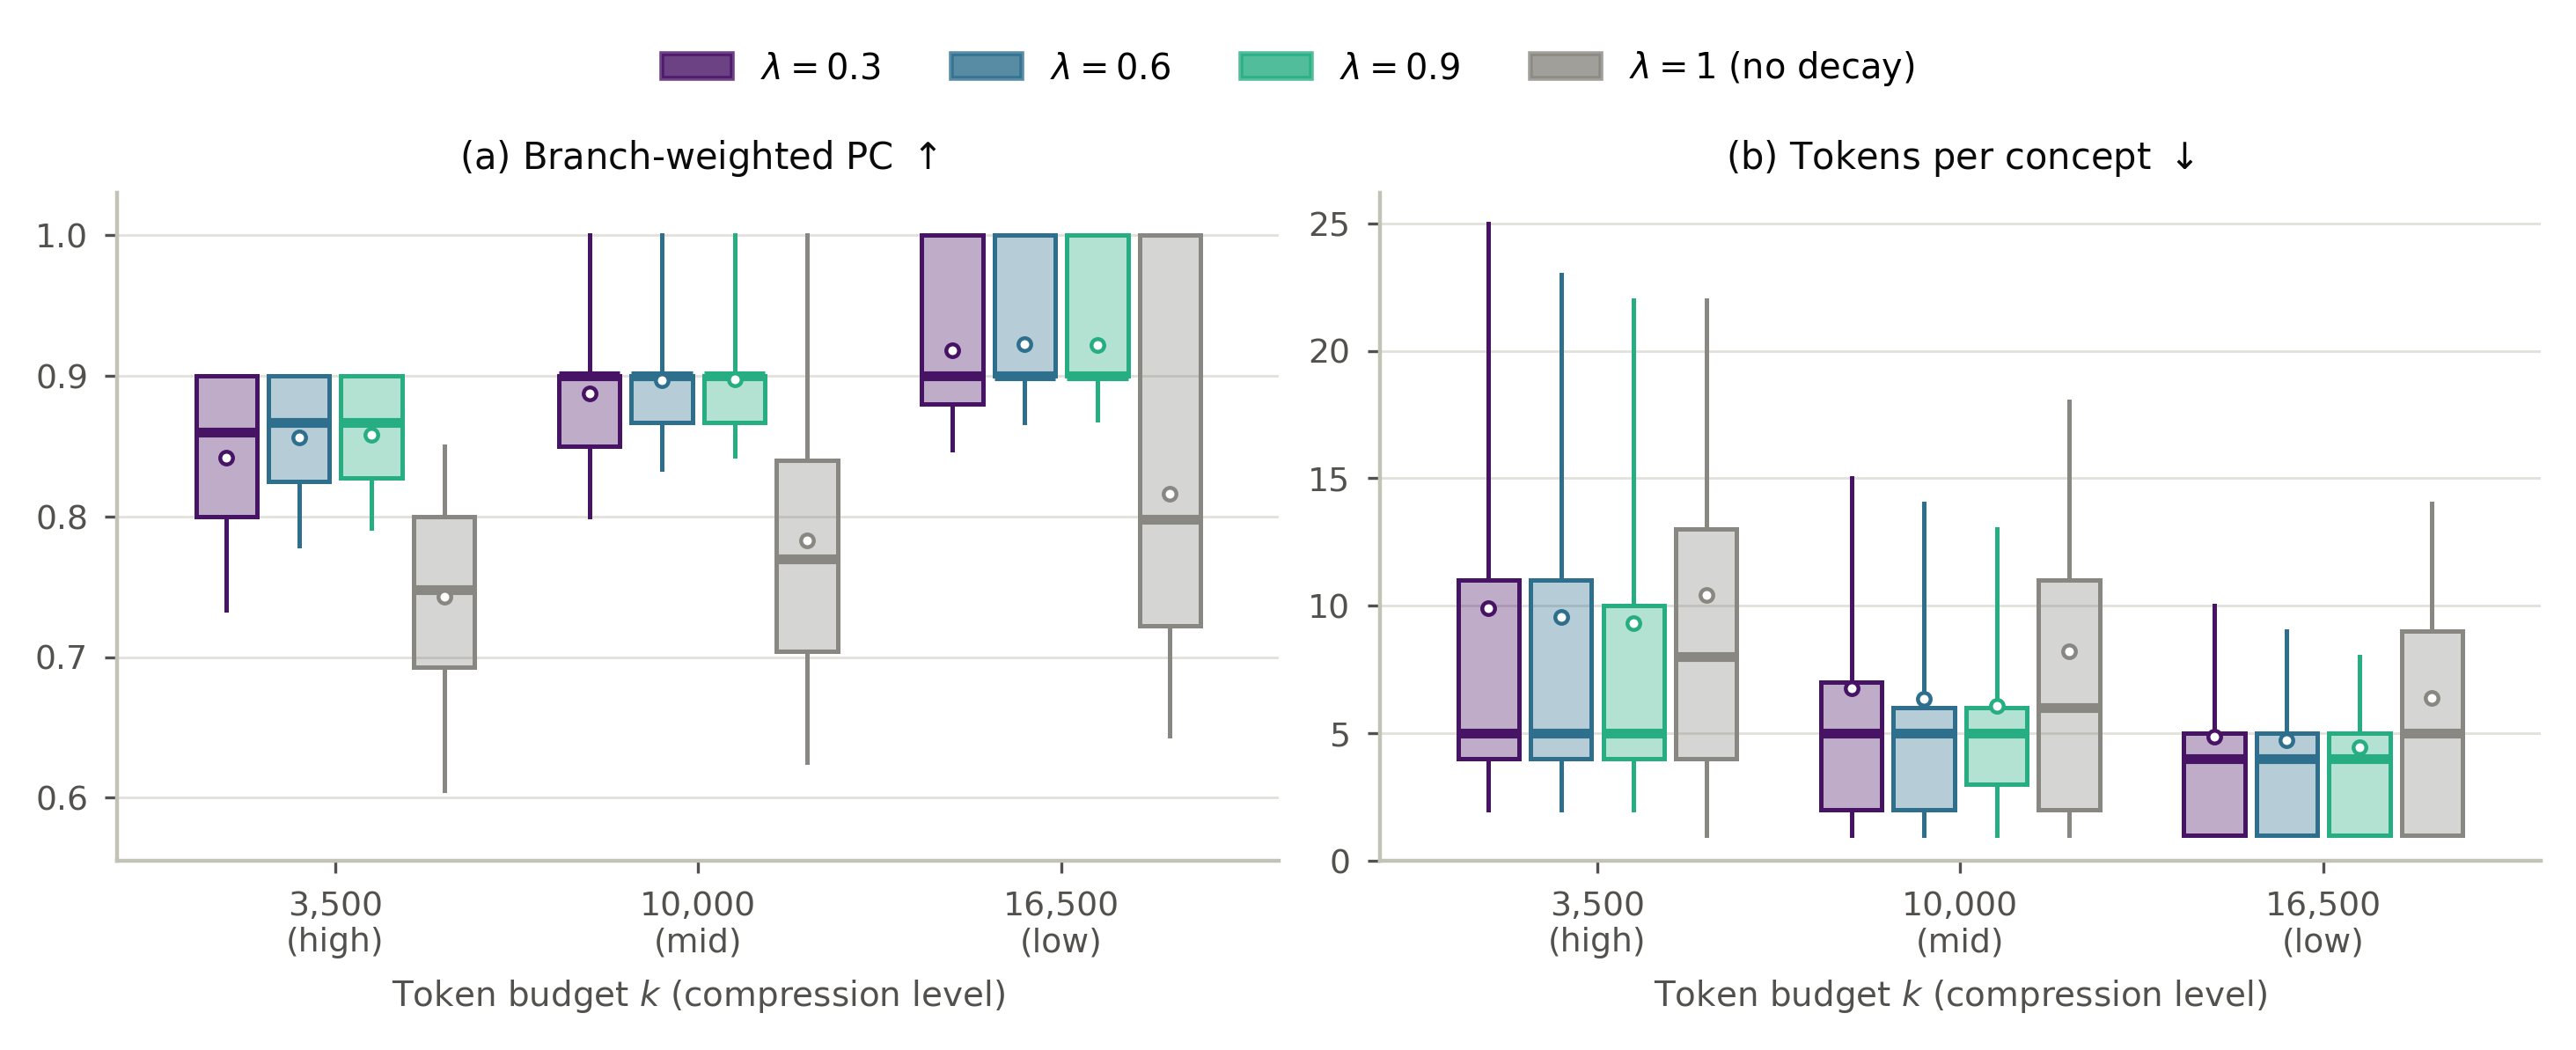
\includegraphics[width=\textwidth]{imgs/dist_k_lambda.png}
\caption{Per-concept scores of our method on the mapped concepts $M$, at one token budget per compression level ($k/|M| = 7.6\%$, $21.7\%$ and $35.8\%$) and four values of the decay $\lambda$.
(a)~Proximity-coverage score and (b)~tokens per concept: boxes span the 25th to 75th percentiles, thick lines mark the median, whiskers the 10th and 90th percentiles, and dots the mean.
Many concepts score exactly 0.9 (all tokens one hop away) or 1 (the concept is itself a token).
No concept is unknown in these settings, except 0.06\% at $k = 3{,}500$, $\lambda = 0.3$.}
\label{fig:dist-k-lambda}
\end{figure*}

\paragraph{Vocabulary use.}
Our selection also uses almost every token it selects.
A selected token is unused when every concept that reaches it meets another token first.
With $\lambda = 0.9$, 99.6 to 99.7\% of the tokens appear in at least one context tree at every compression level, against 93 to 94\% for Personalized PageRank, and 87 to 95\% for PageRank, closeness centrality, highest degree ($d \le D$) and the set-cover ablation (Table~\ref{tab:ranking_full}).
Rankings that score each candidate independently, and the set-cover ablation, which credits a token for every concept within $D$ hops even when another token is closer, select hubs together with more specific concepts below them; the concepts then stop at the specific tokens and never reach the hub.
Our marginal gain, in contrast, credits a token only on the walks on which it comes first, so a token becomes unused only if later, more specific tokens hide it.
These baselines thus spend 5 to 13\% of their budget on tokens that no concept uses.

In short, distance-aware greedy selection obtains the best average rank and a higher PC score than every baseline at every compression level, ahead of every degree-, centrality- and set-cover-based selection, and wastes almost none of its budget; within our method, a larger budget or a decay closer to (but below) 1 mainly helps the concepts that are worst represented.

% ------------------------------------------------------------------
\subsection{Rare concepts in real EHR data}
\label{sec:results:hero}

The benchmark treats all concepts alike and uses no patient data.
In real EHR data, concept frequencies are long-tailed, so the question is whether the rare concepts keep their meaning.
We compare our tokenizer ($\lambda = 0.9$) with frequency truncation on the concepts of the HERO data (Section~\ref{sec:method:ehr}).
We call a concept rare if it occurs in fewer than 100 events.
Concept usage is long-tailed: of the 16,370 concepts, the 2,000 most frequent account for 99\% of the events (Figure~\ref{fig:hero}a), and the two thirds of the concepts that are rare make up less than 0.1\% of the events (Table~\ref{tab:hero_bins}).

\paragraph{Representation of rare concepts.}
Our tokenizer represents rare concepts even with a small token budget.
We take $k = 5{,}000$ as an example; this vocabulary is selected on $\Mhero$ and is unrelated to the benchmark vocabulary of the same size.
At this budget, truncation represents almost every event (Figure~\ref{fig:hero}a) but keeps no rare concept, so every event of a rare concept becomes the unknown token.
Our tokenizer represents every concept, in every frequency bin (Table~\ref{tab:hero_bins}).
The rare concepts also keep most of their meaning: their mean PC score is 0.88, against 0 under truncation, close to that of the frequent concepts.
Personalized PageRank, the best graph baseline, also represents every rare concept at this budget, with a slightly lower mean PC score (0.86).
They borrow strength from frequent concepts: since tokens are shared, the least frequent token of a rare concept occurs in a median of 609 events, whereas the concept itself occurs in a median of 8 (Table~\ref{tab:longtail}).
Nearly every token serves the data: 4,991 of the 5,000 tokens appear in the tree of at least one concept, against 4,692 for Personalized PageRank, so almost no embedding would be left without training events.
The same holds at every budget (Figure~\ref{fig:hero}b and Table~\ref{tab:ehr}): truncation keeps a rare concept only after all 5,761 concepts with at least 100 events, whereas our tokenizer represents virtually all rare concepts from the smallest budget on.

\paragraph{Trade-off with sequence length.}
Our tokenizer represents each concept by a context tree of tokens, and thus produces longer sequences (Figure~\ref{fig:hero}c).
Truncation encodes each event with one token, whereas our tokenizer needs 5.6 tokens per event at $k = 5{,}000$.
This cost falls as $k$ grows, because each branch of a context tree meets a token sooner.
In sum, truncation keeps the events but discards the rare concepts; our tokenizer keeps every concept, with most of its meaning, at the cost of longer sequences.

\begin{figure}[t]
\centering
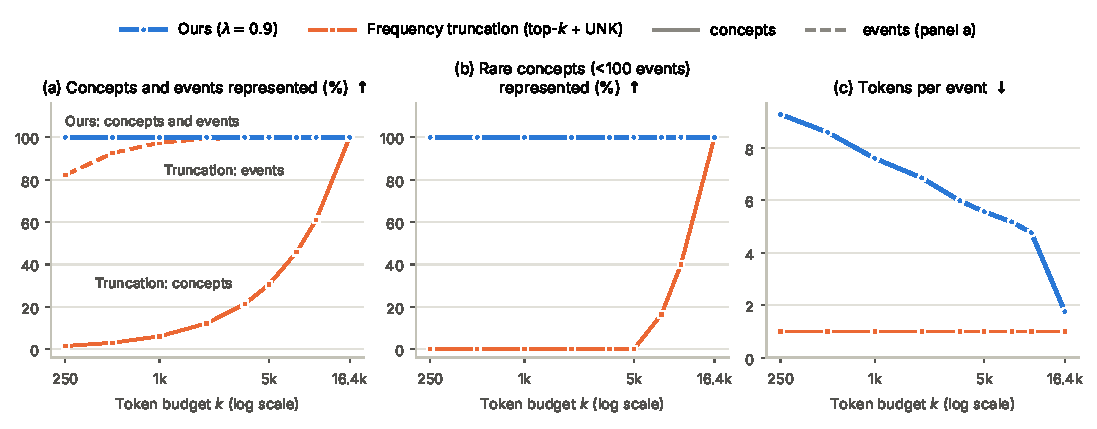
\includegraphics[width=\textwidth]{imgs/ehr_rare_summary.pdf}
\caption{Our tokenizer ($\lambda = 0.9$) and frequency truncation on the HERO data, against the token budget $k$ (log scale; $k = |\Mhero| = 16{,}370$ keeps every concept). (a)~Concepts (solid) and events (dashed) represented by at least one token other than the unknown token. (b)~Rare concepts (fewer than 100 events) represented. (c)~Tokens per event; truncation always costs one. Values for every budget are in Table~\ref{tab:ehr} (Appendix~\ref{app:hero}).}
\label{fig:hero}
\end{figure}

\begin{table}[t]
\centering
\small
\setlength{\tabcolsep}{4pt}
\begin{tabular}{@{}lrrrrrrrr@{}}
\toprule
 & & & \multicolumn{2}{c}{Represented (\%)} & \multicolumn{2}{c}{PC score} & \multicolumn{2}{c}{Median events} \\
\cmidrule(lr){4-5}\cmidrule(lr){6-7}\cmidrule(l){8-9}
Events & Concepts & Events (\%) & Ours & Trunc. & Ours & Trunc. & Concept & Rarest token \\
\midrule
$<10$             & 5,706  & $<$0.1 & 100.0 & 0.0   & 0.88 & 0.00 & 3     & 535    \\
$[10, 100)$       & 4,903  & 0.1    & 100.0 & 0.0   & 0.88 & 0.00 & 28    & 763    \\
$[100, 1{,}000)$  & 3,246  & 0.4    & 100.0 & 76.6  & 0.89 & 0.77 & 261   & 1,759  \\
$\geq 1{,}000$    & 2,515  & 99.5   & 100.0 & 100.0 & 0.90 & 1.00 & 6,485 & 61,017 \\
\midrule
Rare ($<100$)     & 10,609 & 0.1    & 100.0 & 0.0   & 0.88 & 0.00 & 8     & 609    \\
All               & 16,370 & 100.0  & 100.0 & 30.5  & 0.88 & 0.31 & 28    & 1,322  \\
\bottomrule
\end{tabular}
\caption{Concepts of the HERO data grouped by their number of events, at $k = 5{,}000$ and $\lambda = 0.9$. Rare concepts have fewer than 100 events (first two rows). Events (\%): share of all events. Represented: concepts that receive at least one token other than the unknown token. PC score: mean proximity-coverage score; under truncation, a kept concept scores 1 and a discarded one 0. Median events: of the concept, and of the least frequent token in its context tree (ours).}
\label{tab:hero_bins}
\end{table}

% ------------------------------------------------------------------
\subsection{Expert evaluation}
\label{sec:results:expert}

The PC score measures distance in the graph, not clinical meaning, so we asked semanticians whether our trees preserve the meaning of a concept better than those of Personalized PageRank.
Of the 11,796 concepts of the official release, 4,306 have the same tree under both methods, or are kept as a token by both, and count as ``no clear difference'' (Table~\ref{tab:expert-strata}).
\needresults{share of the rated concepts for which experts prefer ours / no clear difference / the baseline, per category and weighted (Table~5, Figure~8); sign test and confidence interval}
\needresults{problems flagged per method: incorrect or ambiguous, absent, precision lost, redundant}
\needresults{agreement between raters; agreement between expert preference and the PC difference}

\section{Discussion}
\label{sec:discussion}

\subsection{Why distance-aware greedy selection preserves meaning}
\label{sec:discussion:why}

Degree- and centrality-based methods score each candidate once, by its position in the graph, independently of the tokens already selected.
They favour hubs near the top of the hierarchy, such as \textit{Qualifier value}, \textit{Action} or \textit{Body structure}, which many concepts reach but which describe none of them well.
Branches then end at generic tokens far from the concept: the PC score drops, and since a long branch fans out over more parents and attributes before it stops, the trees grow longer.
The PC score is the metric on which every baseline falls behind our method: at every budget, any $\lambda$ from 0.4 to 0.9 gives a higher PC score than every baseline (Section~\ref{sec:results:benchmark}).

Our selection starts from similar hubs, with \textit{Qualifier value}, \textit{Body structure} and \textit{Organism} among its first tokens, but it combines two mechanisms that the baselines lack.
The distance decay rewards a token for reaching concepts in few hops, so a token closer to a concept than an already selected hub still raises that concept's coverage.
Marginal-gain selection accounts for the tokens already chosen, so a candidate that only reaches well-covered concepts is passed over; this is also why almost every selected token ends up in some context tree, whereas the baselines spend up to 13\% of their budget on tokens that no concept uses.
After a few hubs, the selection therefore turns to more specific concepts.
Both mechanisms are needed: the set-cover ablation keeps marginal-gain selection but drops the decay, and every $\lambda > 0$ outranks it.

The decay must lie strictly between 0 and 1, because at both extremes the marginal gain stops distinguishing between candidates.
At $\lambda = 0$, only exact matches count: every concept not yet selected has the same gain, the choice is left to the tie-break, and at high compression most concepts receive no token.
At $\lambda = 1$, a token counts the same at any distance: once every walk from the concepts reaches some token, which happens after fewer than 1,000 tokens on $M$, every remaining candidate has zero gain, and the rest of the budget is filled without regard to distance.
Any $\lambda$ strictly between 0 and 1 avoids both failures, and because greedy selection depends on the order of the gains rather than on their size, even a value just below 1 keeps closer tokens ahead of farther ones.
In our benchmark, intermediate values of $\lambda$ thus select tokens that are general enough to be shared by many concepts, yet close enough to each of them to keep its specific relationships.

\subsection{Implications for EHR foundation models}
\label{sec:discussion:ehr}

\paragraph{Rare concepts.}
Frequency truncation and our tokenizer handle the long tail in opposite ways.
Truncation keeps almost all events but maps most distinct concepts, including every rare one, to the unknown token (Section~\ref{sec:results:hero}).
Rare concepts can nevertheless include clinically important conditions and procedures.
Our tokenizer keeps every concept and writes each rare one with tokens it shares with frequent, related concepts.
This is meant to address the learnability problem of the Introduction: a rare concept is written with tokens that occur far more often than the concept itself, in a median of 609 events against 8, although some rare concepts gain nothing (Table~\ref{tab:longtail}).
Whether a model learns better representations of rare concepts from such tokens, and whether this improves downstream clinical predictions, remains to be tested by pretraining experiments.

\paragraph{Sequence length.}
The price is longer sequences: several tokens per event instead of one, and the cost of standard self-attention grows quadratically with sequence length \cite{vaswani2017attention}.
This cost can be reduced by pooling the tokens of each event into a single input position, or by a hybrid vocabulary that keeps the most frequent concepts as their own tokens and spends the rest of the budget on our objective, so that routine events cost one token while rare concepts keep a structured representation.
Whether a model needs the relationship markers of the context tree, or whether flat token sets suffice, is an empirical question; the markers matter most at small budgets, for instance to bind each laterality to its finding site.

\paragraph{Choosing $k$ and $\lambda$.}
The token budget is bounded from two sides.
Each token needs enough training occurrences for its embedding to be learned, and a larger $k$ adds specific tokens shared by fewer concepts, so the tokens of rare concepts occur in fewer events (Table~\ref{tab:ehr}); smaller datasets therefore call for smaller budgets.
Conversely, a smaller vocabulary lengthens the trees and the sequences, so the available compute limits how far the vocabulary can be compressed.
For data of our size, about 280 million events, budgets between 2,000 and 5,000, that is 12\% to 31\% of the concepts, balance the two bounds: at least 94\% of the rare concepts are encoded only by tokens seen in at least 10 events, while an event costs 5.6 to 6.9 tokens.
The decay matters much less: we recommend $\lambda = 0.9$, the best-ranked value at every compression level, and advise against $\lambda = 1$, which looks like the natural choice of no decay but removes the incentive to select close tokens.
Tuning is cheap: one run of the selection gives the vocabulary for every budget, and since it needs only the ontology and the list of concepts, not patient data, the vocabulary can be computed and shared outside the clinical data environment.

\section{Limitations and future work}
\label{sec:limitations}

\paragraph{What the graph does not state cannot be preserved.}
The context trees and the coverage objective only reflect the relationships encoded in the ontology.
This matters most for primitive concepts, whose relationships do not fully define them (Section~\ref{sec:snomed}), and SNOMED~CT has many of them: 64\% of the 420,716 concepts of the release we use are primitive, and in the HERO data, 42\% of the 11,796 concepts that belong to the release are primitive and carry 88\% of the events of these 11,796 concepts.
When a primitive concept is not itself a token, its tree loses the part of its meaning that no relationship states; \textit{hyperthyroidism} and \textit{sick-euthyroid syndrome}, two primitive concepts with the same relationships, receive the same tree (Section~\ref{sec:results:examples}).
The status-dependent decay of Eq.~\eqref{eq:coverage-status} addresses this directly, since it charges exactly the hops where meaning can be lost; evaluating it is our next step.
Two further simplifications come from our design rather than from the graph: all relationship types weigh the same in the objective, and context trees do not record how SNOMED~CT groups the attributes of a concept.
Factors that depend on the relationship type fit the same framework (Section~\ref{sec:method:score}).

\paragraph{Transductive and greedy selection.}
The selection optimizes the coverage of a fixed set of concepts.
A new concept can still be tokenized with an existing vocabulary, since Algorithm~\ref{alg:expand} applies to any concept of the graph, but the vocabulary was not chosen to cover it; a new institution or release may require a new run, which is inexpensive and needs no patient data.
The selection also never removes a token, so hubs selected early remain even when later, more specific tokens cover the same concepts.
The guarantee of Eq.~\eqref{eq:guarantee} bounds the resulting loss in coverage, but not in the other metrics; a pass that swaps out tokens with a small marginal loss could reduce this redundancy.

\paragraph{No downstream or external validation.}
We evaluate the tokenization intrinsically, with the metrics of Section~\ref{sec:method:metrics} and with semanticians on 100 concepts, not on a downstream clinical task.
Whether a foundation model trained on our vocabulary predicts clinical outcomes better than one trained on the full or truncated vocabulary remains to be tested by pretraining experiments.
All data also come from a single institution, whose mapping practice and concept distribution may differ elsewhere.
Where mappings between ontologies exist, the same mechanism could also write the concepts of one terminology with tokens of another.

\paragraph{Graph assumptions.}
The method assumes that edges point from a concept to the concepts that describe it, and that the graph is acyclic (Section~\ref{sec:method:problem}).
Because every traversal is bounded by $D$, it still terminates on a graph with cycles, but on a vocabulary with cycles or symmetric relationships, or on a general knowledge graph, the tokens reached from a concept need not describe it.

\section{Conclusion}
\label{sec:conclusion}

We presented an ontology-based tokenizer that represents clinical concepts with a compact vocabulary of ontology concepts, selected by distance-aware greedy coverage and used through context trees.
On 46,150 mapped concepts, it ranked first among 19 configurations at every compression level, and on real EHR data it represented every concept of the ontology graph, including the rare concepts that frequency truncation discards, with a mean proximity-coverage score of 0.88 for these rare concepts.
\needresults{one sentence on the expert result}
Whether these vocabularies improve EHR foundation models is the next test.


\bibliographystyle{plain}
\bibliography{references}

\appendix
% \appendix is already called in main.tex

\section{Submodularity of the coverage objective}
\label{app:submodular}

Fix a concept $m \in M$ and consider a random walk $w = (w_0, \dots, w_L)$ on $G_D$ that starts at $w_0 = m$, follows a uniformly chosen outgoing edge at each step, and stops after $D$ steps or at a concept without outgoing edges.
The distribution of $w$ does not depend on $T$, and by acyclicity the walk never visits a concept twice.
Let $\pi_j = \prod_{i=1}^{j} \lambda(w_i)$ be the factor accumulated after $j$ hops, with $\lambda(v) = \lambda$ for every $v$ under the uniform decay of Eq.~\eqref{eq:coverage} (so $\pi_j = \lambda^j$) and $\lambda(v) \in [0, 1]$ under the status-dependent decay of Eq.~\eqref{eq:coverage-status}.
Unrolling the recursion gives
\[
S_D(m, T) = \mathbb{E}_w\big[\, g_w(T) \,\big], \qquad g_w(T) = \max_{j \,:\, w_j \in T} \pi_j ,
\]
with $g_w(T) = 0$ if the walk visits no token.
Since every factor is at most 1, $\pi_j$ never increases with $j$, so the maximum is attained at the first token visited, which is where the recursion stops.
For a fixed walk, $g_w$ assigns to each visited concept a non-negative weight and returns the largest weight among the selected tokens.
Such a maximum of non-negative weights is normalized, monotone and submodular \cite{krause2014submodular}.
These properties are preserved under non-negative linear combinations, hence under the expectation over $w$ and the average over $m \in M$, so $F_D$ is normalized, monotone and submodular for any factors in $[0, 1]$.

\section{Notation and selection algorithms}
\label{app:notation}
\label{app:algorithms}

\begin{table}[h]
\centering
\small
\begin{tabular}{@{}ll@{}}
\toprule
\textbf{Symbol} & \textbf{Meaning} \\
\midrule
$G = (V, E)$, $\mathcal{R}$ & ontology as a DAG with typed edges $E \subseteq V \times \mathcal{R} \times V$; relationship types \\
$d(u, v)$ & hop distance from $u$ to $v$ \\
$M$, $\Mhero$ & concepts to represent: mapped concepts; concepts of the HERO data \\
$r$, $D$ & root concept; hop radius \\
$V_D$, $G_D = (V_D, E_D)$ & candidate pool and the subgraph it induces \\
$\mathrm{Out}(u)$, $\mathrm{In}(u)$, $\deg^+(u)$ & outgoing and incoming edges of $u$ in $G_D$; out-degree \\
$T$, $k$ & token set; token budget $k = |T|$ \\
$\lambda$, $\lambda(v)$ & distance decay; status-dependent factor of a hop into $v$ \\
$h$, $S_h(u, T)$ & horizon; semantic coverage of $u$ by $T$ at horizon $h$ \\
$F_D(T)$ & selection objective, mean of $S_D(m, T)$ over $M$ \\
$\Delta(t \mid T)$ & marginal gain of adding $t$ to $T$ \\
$n_m$, $u_m$ & tokens and uncovered branches in the context tree of $m$ \\
$\phi(u, \ell)$ & score of concept $u$ reached after $\ell$ hops, Eq.~\eqref{eq:pc} \\
$\omega_b$, $\ell_b$, $B^{+}_m$ & weight and depth of a branch $b$; branches of $m$ that end at a token \\
$c_m$, $p_m$, $\mathrm{PC}_m$ & branch coverage, proximity and proximity-coverage score of $m$ \\
$\sigma_m$, $N_s$ & signature of the tree of $m$; number of concepts with signature $s$ \\
\bottomrule
\end{tabular}
\caption{Notation.}
\label{tab:notation}
\end{table}

Algorithm~\ref{alg:select-tokens} gives the lazy greedy selection of Section~\ref{sec:method:selection}, and Algorithm~\ref{alg:candidate-delta} the incremental computation of a marginal gain.
\textsc{CandidateDelta}$(t)$ propagates the change caused by adding $t$ backward along incoming edges, one hop per round, and touches only the concepts that reach $t$ within $D$ hops.
The initial pass makes $|V_D|$ independent calls, which can run in parallel, and builds the heap in $O(|V_D| \log |V_D|)$.
Each later step costs one or more calls and $O(\log |V_D|)$ heap operations; in the worst case, every candidate is re-evaluated at every step, which gives the $O(k \cdot |V_D|)$ calls of plain greedy.

\begin{algorithm}[h]
\caption{\textsc{SelectTokens}: lazy greedy token selection.}
\label{alg:select-tokens}
\begin{algorithmic}[1]
\Require candidate pool $V_D$, concepts $M$, hop radius $D$, token budget $k$, distance decay $\lambda$
\Ensure token set $T$ with $|T| = k$ (or fewer if candidates run out)
\State $T \gets \varnothing$;\ $S \gets \mathbf{0}$;\ $H \gets$ empty max-heap \Comment{$S_h(u)$ stores $S_h(u, T)$}
\ForAll{$t \in V_D$} \Comment{initial pass: exact gains, parallelizable}
    \State $(\mathrm{gain}, \_) \gets \Call{CandidateDelta}{t}$
    \State push $(t, \mathrm{gain})$ onto $H$
\EndFor
\While{$|T| < k$ \textbf{and} $H \neq \varnothing$}
  \State $t \gets$ pop top of $H$
  \State $(\mathrm{gain}, \delta) \gets \Call{CandidateDelta}{t}$ \Comment{exact gain, not a stale bound}
  \State $b \gets$ bound at the top of $H$ (or $-\infty$ if $H$ is empty)
  \If{$\mathrm{gain} \geq b$}
    \State $\Call{Commit}{t, \delta}$ \Comment{by submodularity, no stale bound can beat it}
  \Else
    \State push $(t, \mathrm{gain})$ onto $H$ \Comment{refreshed bound}
  \EndIf
\EndWhile
\State \Return $T$
\end{algorithmic}
\end{algorithm}

\begin{algorithm}[h]
\caption{\textsc{CandidateDelta} and \textsc{Commit}: incremental update. Dictionary entries that are not set are zero.}
\label{alg:candidate-delta}
\begin{algorithmic}[1]
\Function{CandidateDelta}{$t$}
    \State $\delta_0 \gets \{\, t \mapsto 1 - S_0(t) \,\}$ \Comment{only $t$ changes at horizon $0$}
    \For{$h = 1, \dots, D$}
        \State $\delta_h \gets \{\}$
        \ForAll{$v$ with $\delta_{h-1}[v] \neq 0$}
            \ForAll{$(u, R, v) \in \mathrm{In}(v)$ with $u \notin T \cup \{t\}$}
                \State $\delta_h[u] \gets \delta_h[u] + \lambda\, \delta_{h-1}[v] / \deg^+(u)$ \Comment{Eq.~\eqref{eq:coverage}, backward}
            \EndFor
        \EndFor
        \State $\delta_h[t] \gets 1 - S_h(t)$ \Comment{$t$ is absorbing at every horizon}
    \EndFor
    \State $\mathrm{gain} \gets \frac{1}{|M|} \sum_{m \in M \,:\, \delta_D[m] \neq 0} \delta_D[m]$
    \State \Return $(\mathrm{gain}, \delta)$
\EndFunction
\Function{Commit}{$t$, $\delta$}
    \For{$h = 0, \dots, D$}
        \ForAll{$u$ with $\delta_h[u] \neq 0$}
            \State $S_h(u) \gets S_h(u) + \delta_h[u]$
        \EndFor
    \EndFor
    \State $T \gets T \cup \{t\}$
\EndFunction
\end{algorithmic}
\end{algorithm}

\section{Relationship types absent from the candidate subgraph}
\label{app:relations}

Of the 113 relationship types of the full graph $G$, 103 occur in the candidate subgraph $G_D$ of the benchmark.
The other 10 (Table~\ref{tab:omitted-relations}) connect no two concepts of $V_D$.

\begin{table}[h]
\centering
\small
\begin{tabular}{@{}ll@{}}
\toprule
has absorbability                   & measurement method  \\
has coating material                & process extends to  \\
has filling                         & regional part of    \\
has ingredient qualitative strength & relative to part of \\
has surface texture                 & towards             \\
\bottomrule
\end{tabular}
\caption{Relationship types present in $G$ but absent from $G_D$ ($D = 9$). Most describe physical objects or medicinal products, which rarely occur in the mapped clinical data.}
\label{tab:omitted-relations}
\end{table}

\section{Full ranking and effect of the distance decay}
\label{app:ranking}
\label{app:lambda}

Table~\ref{tab:ranking_full} gives the per-metric ranks behind Figure~\ref{fig:rank-by-family}.
Table~\ref{tab:lambda} and Figure~\ref{fig:metrics-vs-lambda} give the mean metrics of our method for every value of $\lambda$.

\begin{table}[p]
\centering
\footnotesize
\caption{Ranking of the 19 configurations on the mapped concepts $M$. At each budget $k$, configurations are ranked on each metric (1 = best; ties share their mean rank). Ranks are averaged over the 13 budgets of each level. \emph{Avg.}\ is the mean over the four core metrics; rows are sorted by it. Bold: best value in the column and level, omitted when most configurations tie. PC: proximity-coverage score; Uniq.: unique rate; Unk.: unknown rate; Tok.: tokens per concept. \emph{Used} is not ranked: it is the vocabulary use, the share of the $k$ selected tokens that appear in at least one context tree, averaged over the budgets of the level.}
\label{tab:ranking_full}
\begin{tabular}{@{}lcccccc@{}}
\toprule
Configuration & PC $\uparrow$ & Uniq. $\uparrow$ & Unk. $\downarrow$ & Tok. $\downarrow$ & Avg. & Used (\%) \\
\midrule
\multicolumn{7}{@{}l}{\textit{High compression ($k = 500$--$6{,}500$)}} \\
\addlinespace[2pt]
Ours ($\lambda = 0.9$) & \textbf{1.0} & 6.3 & 5.5 & 7.4 & \textbf{5.06} & 99.7 \\
Ours ($\lambda = 0.8$) & 2.0 & 4.8 & 5.9 & 8.2 & 5.25 & 99.8 \\
Ours ($\lambda = 0.7$) & 3.0 & 3.8 & 6.1 & 9.1 & 5.50 & 99.9 \\
Ours ($\lambda = 0.6$) & 4.0 & 2.8 & 7.9 & 10.4 & 6.26 & 99.9 \\
Ours ($\lambda = 0.5$) & 5.0 & \textbf{2.5} & 8.5 & 11.6 & 6.91 & 100.0 \\
Ours ($\lambda = 0.4$) & 6.0 & 4.1 & 9.7 & 12.3 & 8.01 & 100.0 \\
Highest degree, $d \le 1$ & 9.5 & 5.5 & 16.8 & 3.6 & 8.88 & 100.0 \\
Personalized PageRank & 7.0 & 9.2 & 6.0 & 15.2 & 9.35 & 93.4 \\
Ours ($\lambda = 0.3$) & 9.1 & 6.7 & 10.4 & 13.0 & 9.79 & 100.0 \\
Ours ($\lambda = 0.2$) & 11.9 & 9.3 & 11.3 & 8.9 & 10.38 & 100.0 \\
PageRank & 8.8 & 11.1 & 6.3 & 15.8 & 10.47 & 93.3 \\
Closeness centrality & 11.4 & 12.6 & 12.7 & 6.7 & 10.85 & 93.1 \\
Highest degree, $d \le D$ & 12.4 & 13.2 & 13.5 & 6.8 & 11.48 & 93.7 \\
Ours ($\lambda = 0.1$) & 14.1 & 13.0 & 12.4 & 6.5 & 11.50 & 100.0 \\
Ours ($\lambda = 1.0$) & 15.5 & 16.8 & \textbf{5.4} & 14.8 & 13.11 & 99.9 \\
Random & 18.0 & 18.0 & 18.0 & 2.0 & 14.00 & 98.9 \\
Most IS\_A children & 15.5 & 15.0 & 9.1 & 17.7 & 14.34 & 97.6 \\
Set cover (ablation) & 16.8 & 16.2 & \textbf{5.4} & 19.0 & 14.38 & 95.4 \\
Ours ($\lambda = 0.0$) & 19.0 & 19.0 & 19.0 & \textbf{1.0} & 14.50 & 100.0 \\
\midrule
\multicolumn{7}{@{}l}{\textit{Mid compression ($k = 7{,}000$--$13{,}000$)}} \\
\addlinespace[2pt]
Ours ($\lambda = 0.9$) & 2.0 & \textbf{1.8} & 8.5 & 3.6 & \textbf{3.99} & 99.7 \\
Ours ($\lambda = 0.8$) & \textbf{1.2} & 2.4 & 8.5 & 5.3 & 4.36 & 99.8 \\
Ours ($\lambda = 0.7$) & 2.8 & 3.2 & 8.5 & 6.6 & 5.28 & 99.8 \\
Ours ($\lambda = 0.6$) & 4.0 & 4.5 & 8.5 & 7.9 & 6.24 & 99.9 \\
Ours ($\lambda = 0.5$) & 5.0 & 5.9 & 8.5 & 9.2 & 7.14 & 99.9 \\
Personalized PageRank & 7.5 & 3.3 & 8.5 & 11.1 & 7.61 & 93.3 \\
Ours ($\lambda = 0.4$) & 6.0 & 7.6 & 8.5 & 11.2 & 8.32 & 100.0 \\
Highest degree, $d \le 1$ & 8.9 & 7.2 & 17.0 & 2.4 & 8.87 & 99.6 \\
Closeness centrality & 11.6 & 11.2 & 8.5 & 5.2 & 9.14 & 91.0 \\
Ours ($\lambda = 0.3$) & 7.7 & 9.5 & 8.5 & 13.9 & 9.91 & 100.0 \\
Highest degree, $d \le D$ & 12.8 & 12.7 & 8.5 & 5.8 & 9.95 & 90.6 \\
PageRank & 10.4 & 9.5 & 8.5 & 14.4 & 10.68 & 90.0 \\
Ours ($\lambda = 0.2$) & 11.1 & 12.1 & 8.5 & 12.5 & 11.03 & 100.0 \\
Ours ($\lambda = 0.1$) & 14.0 & 14.0 & 8.5 & 13.8 & 12.57 & 100.0 \\
Most IS\_A children & 15.0 & 15.8 & 8.5 & 17.0 & 14.09 & 93.3 \\
Ours ($\lambda = 0.0$) & 19.0 & 19.0 & 19.0 & \textbf{1.0} & 14.50 & 100.0 \\
Ours ($\lambda = 1.0$) & 16.0 & 17.2 & 8.5 & 17.5 & 14.82 & 99.9 \\
Set cover (ablation) & 17.0 & 15.2 & 8.5 & 19.0 & 14.91 & 92.0 \\
Random & 18.0 & 17.8 & 18.0 & 12.6 & 16.60 & 96.8 \\
\midrule
\multicolumn{7}{@{}l}{\textit{Low compression ($k = 13{,}500$--$19{,}500$)}} \\
\addlinespace[2pt]
Ours ($\lambda = 0.9$) & 4.5 & 2.0 & 9.0 & 2.0 & \textbf{4.38} & 99.6 \\
Ours ($\lambda = 0.7$) & \textbf{1.6} & 3.4 & 9.0 & 4.0 & 4.49 & 99.8 \\
Ours ($\lambda = 0.8$) & 2.9 & 3.7 & 9.0 & 3.0 & 4.64 & 99.7 \\
Ours ($\lambda = 0.6$) & 2.1 & 4.9 & 9.0 & 5.2 & 5.28 & 99.9 \\
Ours ($\lambda = 0.5$) & 4.0 & 6.1 & 9.0 & 6.2 & 6.32 & 99.9 \\
Ours ($\lambda = 0.4$) & 5.8 & 8.2 & 9.0 & 7.6 & 7.64 & 100.0 \\
Personalized PageRank & 8.8 & \textbf{1.0} & 9.0 & 12.7 & 7.88 & 94.0 \\
Ours ($\lambda = 0.3$) & 7.0 & 10.3 & 9.0 & 9.2 & 8.86 & 100.0 \\
Highest degree, $d \le 1$ & 10.5 & 6.9 & 9.6 & 8.8 & 8.94 & 97.1 \\
Ours ($\lambda = 0.2$) & 8.2 & 13.0 & 9.0 & 10.1 & 10.05 & 100.0 \\
Closeness centrality & 12.7 & 10.7 & 9.0 & 12.0 & 11.09 & 88.4 \\
PageRank & 11.6 & 8.8 & 9.0 & 15.0 & 11.11 & 87.6 \\
Ours ($\lambda = 0.1$) & 11.5 & 14.0 & 9.0 & 10.2 & 11.14 & 100.0 \\
Highest degree, $d \le D$ & 13.8 & 12.0 & 9.0 & 13.2 & 11.97 & 87.3 \\
Most IS\_A children & 15.0 & 16.1 & 9.0 & 16.8 & 14.22 & 88.5 \\
Ours ($\lambda = 0.0$) & 19.0 & 19.0 & 19.0 & \textbf{1.0} & 14.50 & 100.0 \\
Set cover (ablation) & 16.3 & 15.0 & 9.0 & 18.8 & 14.76 & 87.8 \\
Ours ($\lambda = 1.0$) & 16.7 & 18.0 & 9.0 & 16.2 & 14.95 & 99.7 \\
Random & 18.0 & 16.9 & 18.0 & 18.2 & 17.79 & 94.6 \\
\bottomrule
\end{tabular}
\end{table}

\begin{table}[htbp]
\centering
\caption{Mean metrics of our method for each value of the distance decay $\lambda$ on the mapped concepts $M$, averaged over the 13 token budgets of each compression level. $\lambda = 0.9$ is the default (bold). PC: proximity-coverage score; Uniq.: unique rate; Unk.: unknown rate; Tok.: tokens per concept; Unc.: uncovered branch rate.}
\label{tab:lambda}
\footnotesize
\setlength{\tabcolsep}{4pt}
\begin{tabular}{@{}llrrrrr@{}}
\toprule
Level & $\lambda$ & PC\,$\uparrow$ & Uniq.\,$\uparrow$ & Unk.\,$\downarrow$ & Tok.\,$\downarrow$ & Unc.\,$\downarrow$ \\
\midrule
\multirow{11}{*}{High} & 0.0 & 0.084 & 0.143 & 0.765 & 0.3 & 0.924 \\
 & 0.1 & 0.790 & 0.617 & 0.002 & 9.2 & 0.289 \\
 & 0.2 & 0.817 & 0.681 & 0.001 & 9.6 & 0.233 \\
 & 0.3 & 0.831 & 0.704 & 0.001 & 10.1 & 0.168 \\
 & 0.4 & 0.839 & 0.714 & 0.001 & 10.2 & 0.130 \\
 & 0.5 & 0.843 & 0.717 & $<$0.001 & 10.1 & 0.094 \\
 & 0.6 & 0.845 & 0.716 & $<$0.001 & 10.0 & 0.074 \\
 & 0.7 & 0.847 & 0.714 & $<$0.001 & 9.9 & 0.064 \\
 & 0.8 & 0.848 & 0.711 & $<$0.001 & 9.8 & 0.050 \\
 & \textbf{0.9} & 0.848 & 0.707 & $<$0.001 & 9.8 & 0.042 \\
 & 1.0 & 0.740 & 0.468 & 0.000 & 10.8 & 0.003 \\
\midrule
\multirow{11}{*}{Mid} & 0.0 & 0.234 & 0.298 & 0.493 & 0.7 & 0.782 \\
 & 0.1 & 0.856 & 0.731 & 0.000 & 6.8 & 0.184 \\
 & 0.2 & 0.877 & 0.798 & 0.000 & 6.8 & 0.132 \\
 & 0.3 & 0.887 & 0.823 & 0.000 & 6.8 & 0.081 \\
 & 0.4 & 0.892 & 0.839 & 0.000 & 6.7 & 0.055 \\
 & 0.5 & 0.895 & 0.846 & 0.000 & 6.5 & 0.030 \\
 & 0.6 & 0.896 & 0.850 & 0.000 & 6.4 & 0.021 \\
 & 0.7 & 0.897 & 0.854 & 0.000 & 6.3 & 0.015 \\
 & 0.8 & 0.897 & 0.855 & 0.000 & 6.2 & 0.012 \\
 & \textbf{0.9} & 0.897 & 0.856 & 0.000 & 6.1 & 0.007 \\
 & 1.0 & 0.783 & 0.570 & 0.000 & 8.2 & 0.000 \\
\midrule
\multirow{11}{*}{Low} & 0.0 & 0.403 & 0.480 & 0.210 & 1.5 & 0.636 \\
 & 0.1 & 0.897 & 0.781 & 0.000 & 4.9 & 0.117 \\
 & 0.2 & 0.912 & 0.848 & 0.000 & 4.9 & 0.076 \\
 & 0.3 & 0.918 & 0.872 & 0.000 & 4.9 & 0.043 \\
 & 0.4 & 0.921 & 0.885 & 0.000 & 4.8 & 0.027 \\
 & 0.5 & 0.922 & 0.894 & 0.000 & 4.7 & 0.016 \\
 & 0.6 & 0.922 & 0.900 & 0.000 & 4.6 & 0.011 \\
 & 0.7 & 0.922 & 0.902 & 0.000 & 4.6 & 0.008 \\
 & 0.8 & 0.922 & 0.902 & 0.000 & 4.5 & 0.006 \\
 & \textbf{0.9} & 0.922 & 0.904 & 0.000 & 4.4 & 0.004 \\
 & 1.0 & 0.814 & 0.630 & 0.000 & 6.5 & 0.000 \\
\bottomrule
\end{tabular}
\end{table}

\begin{figure*}[htbp]
\centering
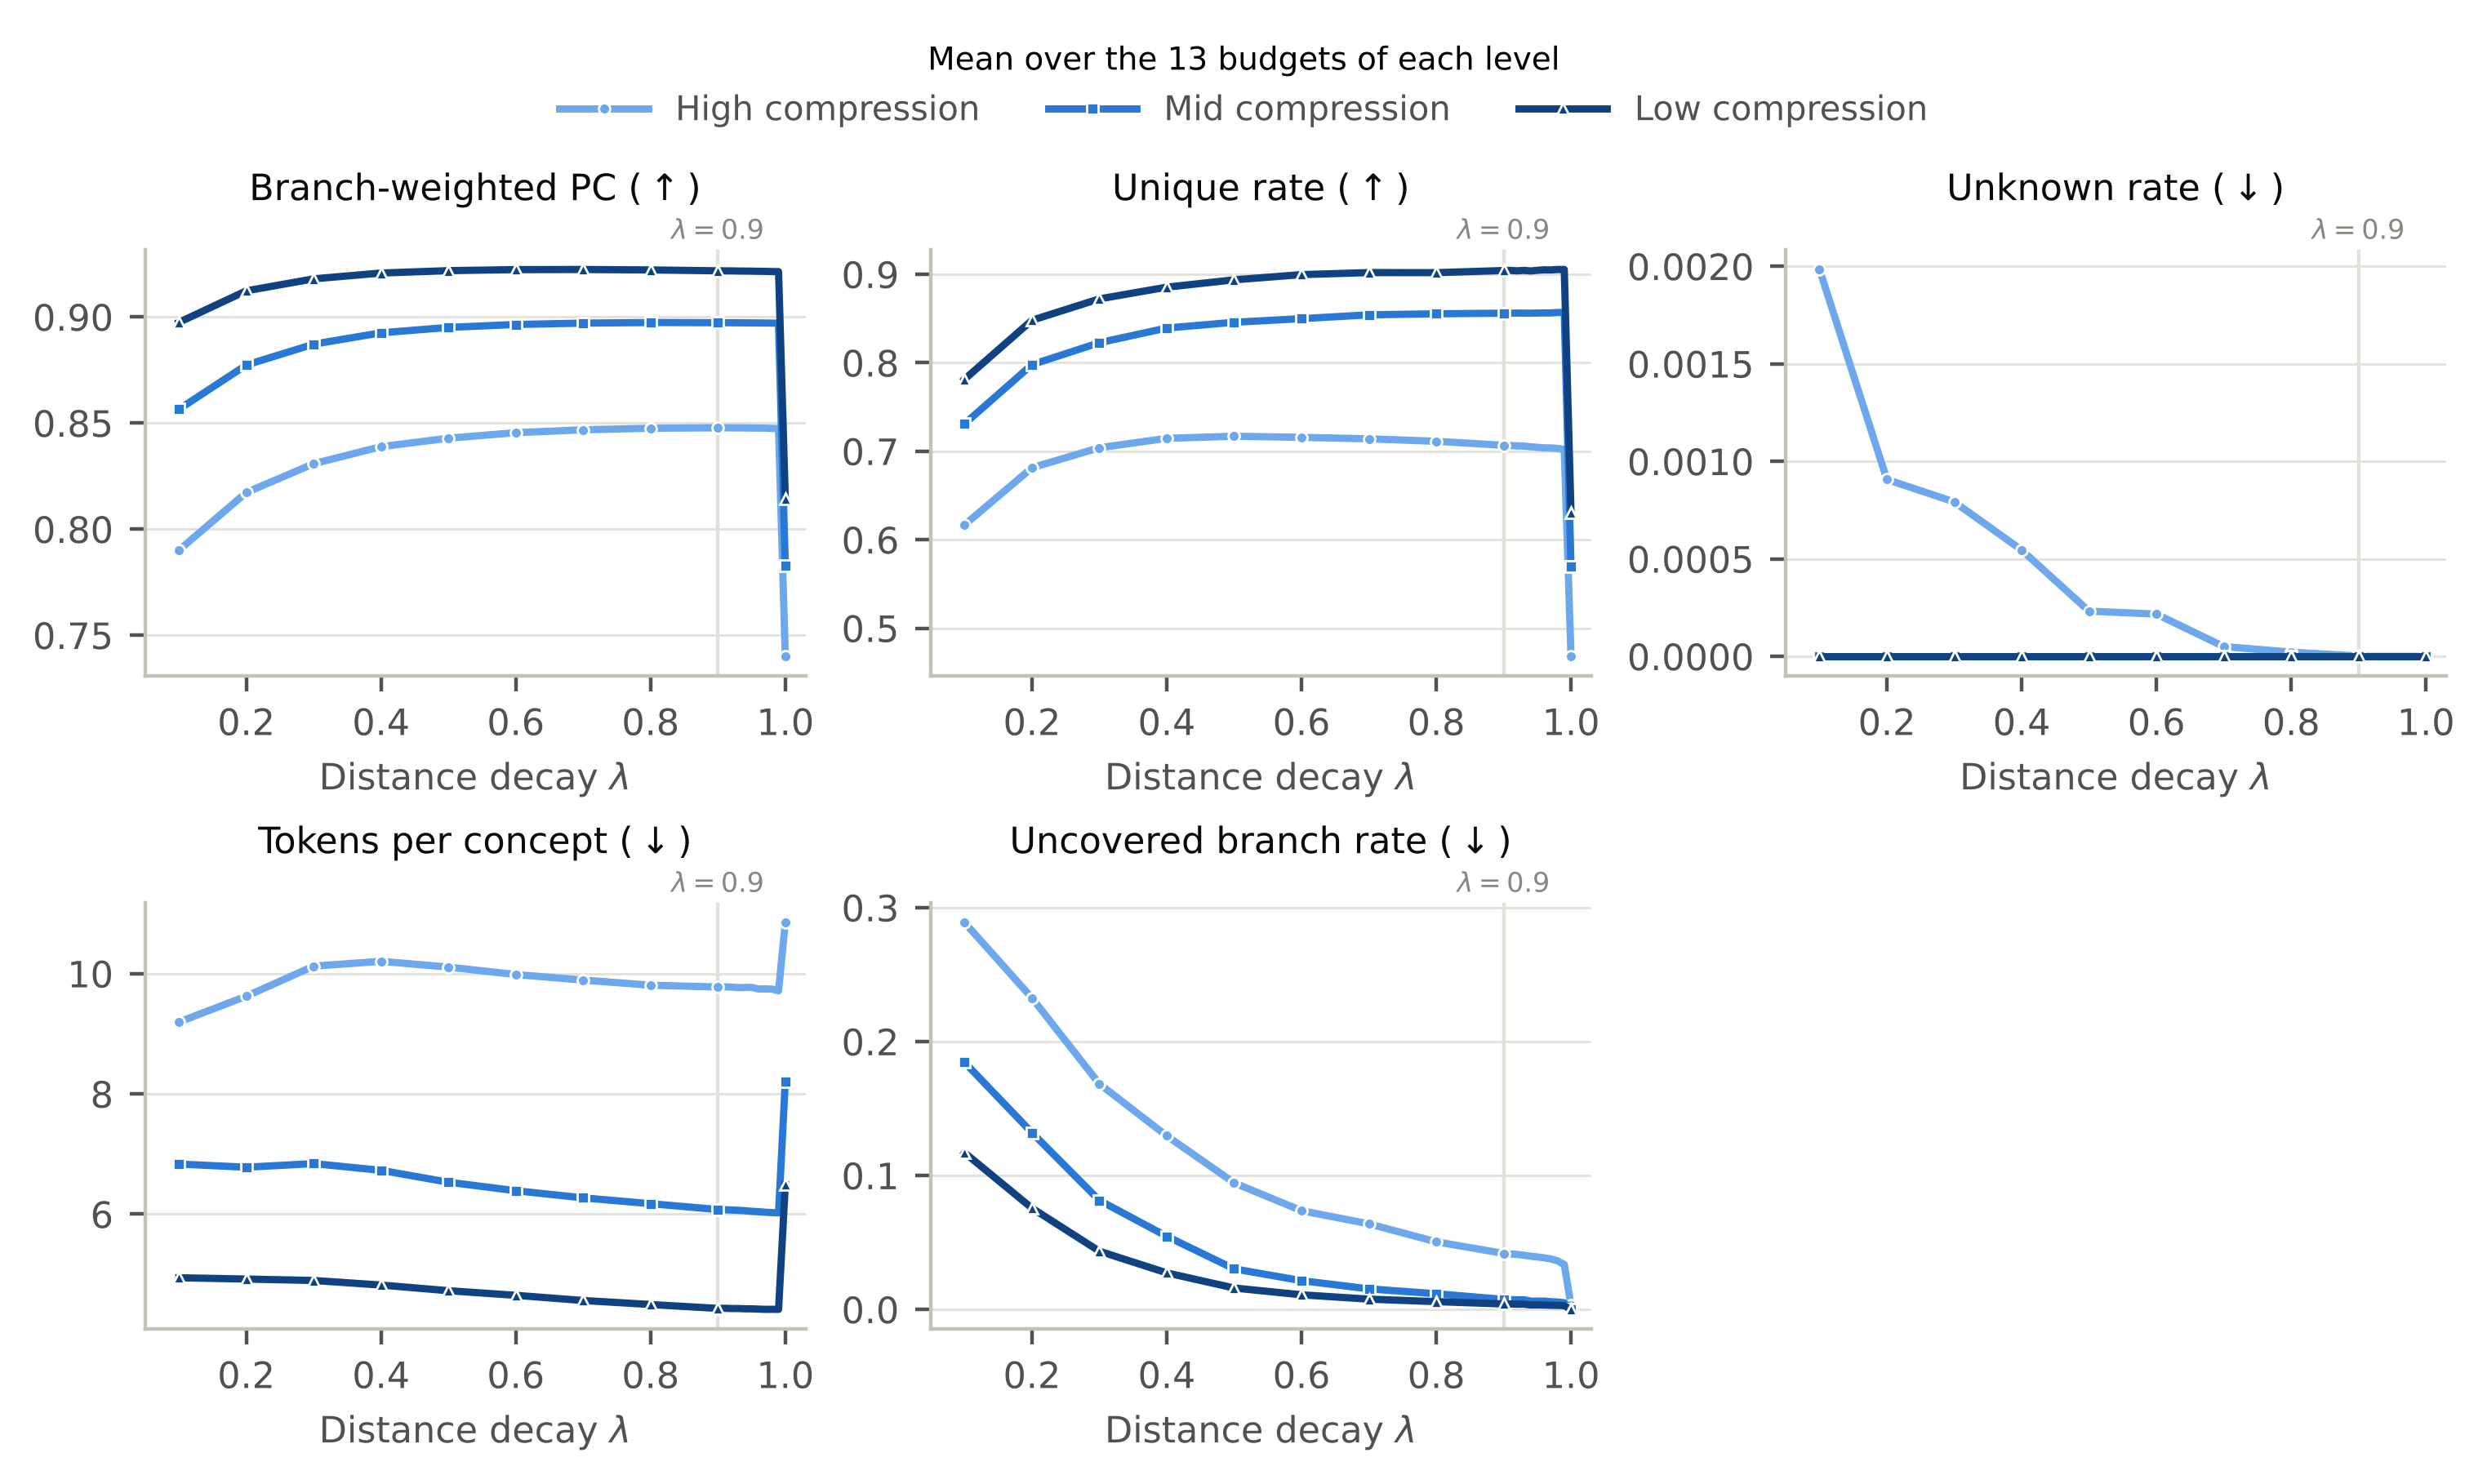
\includegraphics[width=\textwidth]{imgs/metrics_vs_lambda.png}
\caption{Mean metrics of our method as a function of the distance decay $\lambda$, averaged over the 13 token budgets of each compression level.
Lines include $\lambda = 0.91$ to $0.99$; markers show steps of 0.1.
The vertical line marks the default $\lambda = 0.9$.
$\lambda = 0$ is omitted for readability; its values are in Table~\ref{tab:lambda}.}
\label{fig:metrics-vs-lambda}
\end{figure*}

\section{Unweighted proximity-coverage score}
\label{app:flat-pc}

The unweighted PC score is the plain mean of $1 - \ell/(D + 1)$ over the branch ends of the context tree, where an uncovered branch counts as depth $D + 1$:
\[
\mathrm{PC}^{\mathrm{flat}}_m = \frac{1}{n_m + u_m} \Big( \sum_{i=1}^{n_m} \Big(1 - \frac{\ell_i}{D + 1}\Big) \Big),
\]
with $\ell_1, \dots, \ell_{n_m}$ the depths of the tokens of $m$.
It ignores how the branches of a concept fan out (Section~\ref{sec:method:metrics}), but it does not use the walks of the selection objective.
Ranking the 19 configurations with it instead of the weighted score leaves the conclusions unchanged: our method with $\lambda = 0.9$ obtains the best average rank at every compression level, ahead of the same best baselines (Table~\ref{tab:flat-pc}).
Per concept, the two scores agree closely: for $\lambda = 0.9$, their Spearman correlation is 0.86 at $k = 3{,}500$ and 0.94 at $k = 16{,}500$, and they are equal for 49\% and 84\% of the concepts.

\begin{table}[h]
\centering
\small
\setlength{\tabcolsep}{5pt}
\begin{tabular}{@{}lcccc@{}}
\toprule
 & \multicolumn{2}{c}{Weighted PC (main text)} & \multicolumn{2}{c}{Unweighted PC} \\
\cmidrule(lr){2-3}\cmidrule(l){4-5}
Level & Ours ($\lambda = 0.9$) & Best baseline & Ours ($\lambda = 0.9$) & Best baseline \\
\midrule
High & \textbf{5.06} & 8.88 (highest degree, $d \le 1$) & \textbf{5.06} & 8.50 (highest degree, $d \le 1$) \\
Mid  & \textbf{3.99} & 7.61 (Personalized PageRank)      & \textbf{3.74} & 7.34 (Personalized PageRank) \\
Low  & \textbf{4.38} & 7.88 (Personalized PageRank)      & \textbf{3.49} & 7.45 (Personalized PageRank) \\
\bottomrule
\end{tabular}
\caption{Average rank (1 = best) of our method and of the best baseline over the four core metrics, with the weighted PC score of Eq.~\eqref{eq:pc} and with the unweighted one. Bold: best configuration of the level.}
\label{tab:flat-pc}
\end{table}

\section{Metrics as a function of \texorpdfstring{$k$}{k}, including random selection}
\label{app:metrics-vs-k-all}

\begin{figure*}[h]
\centering
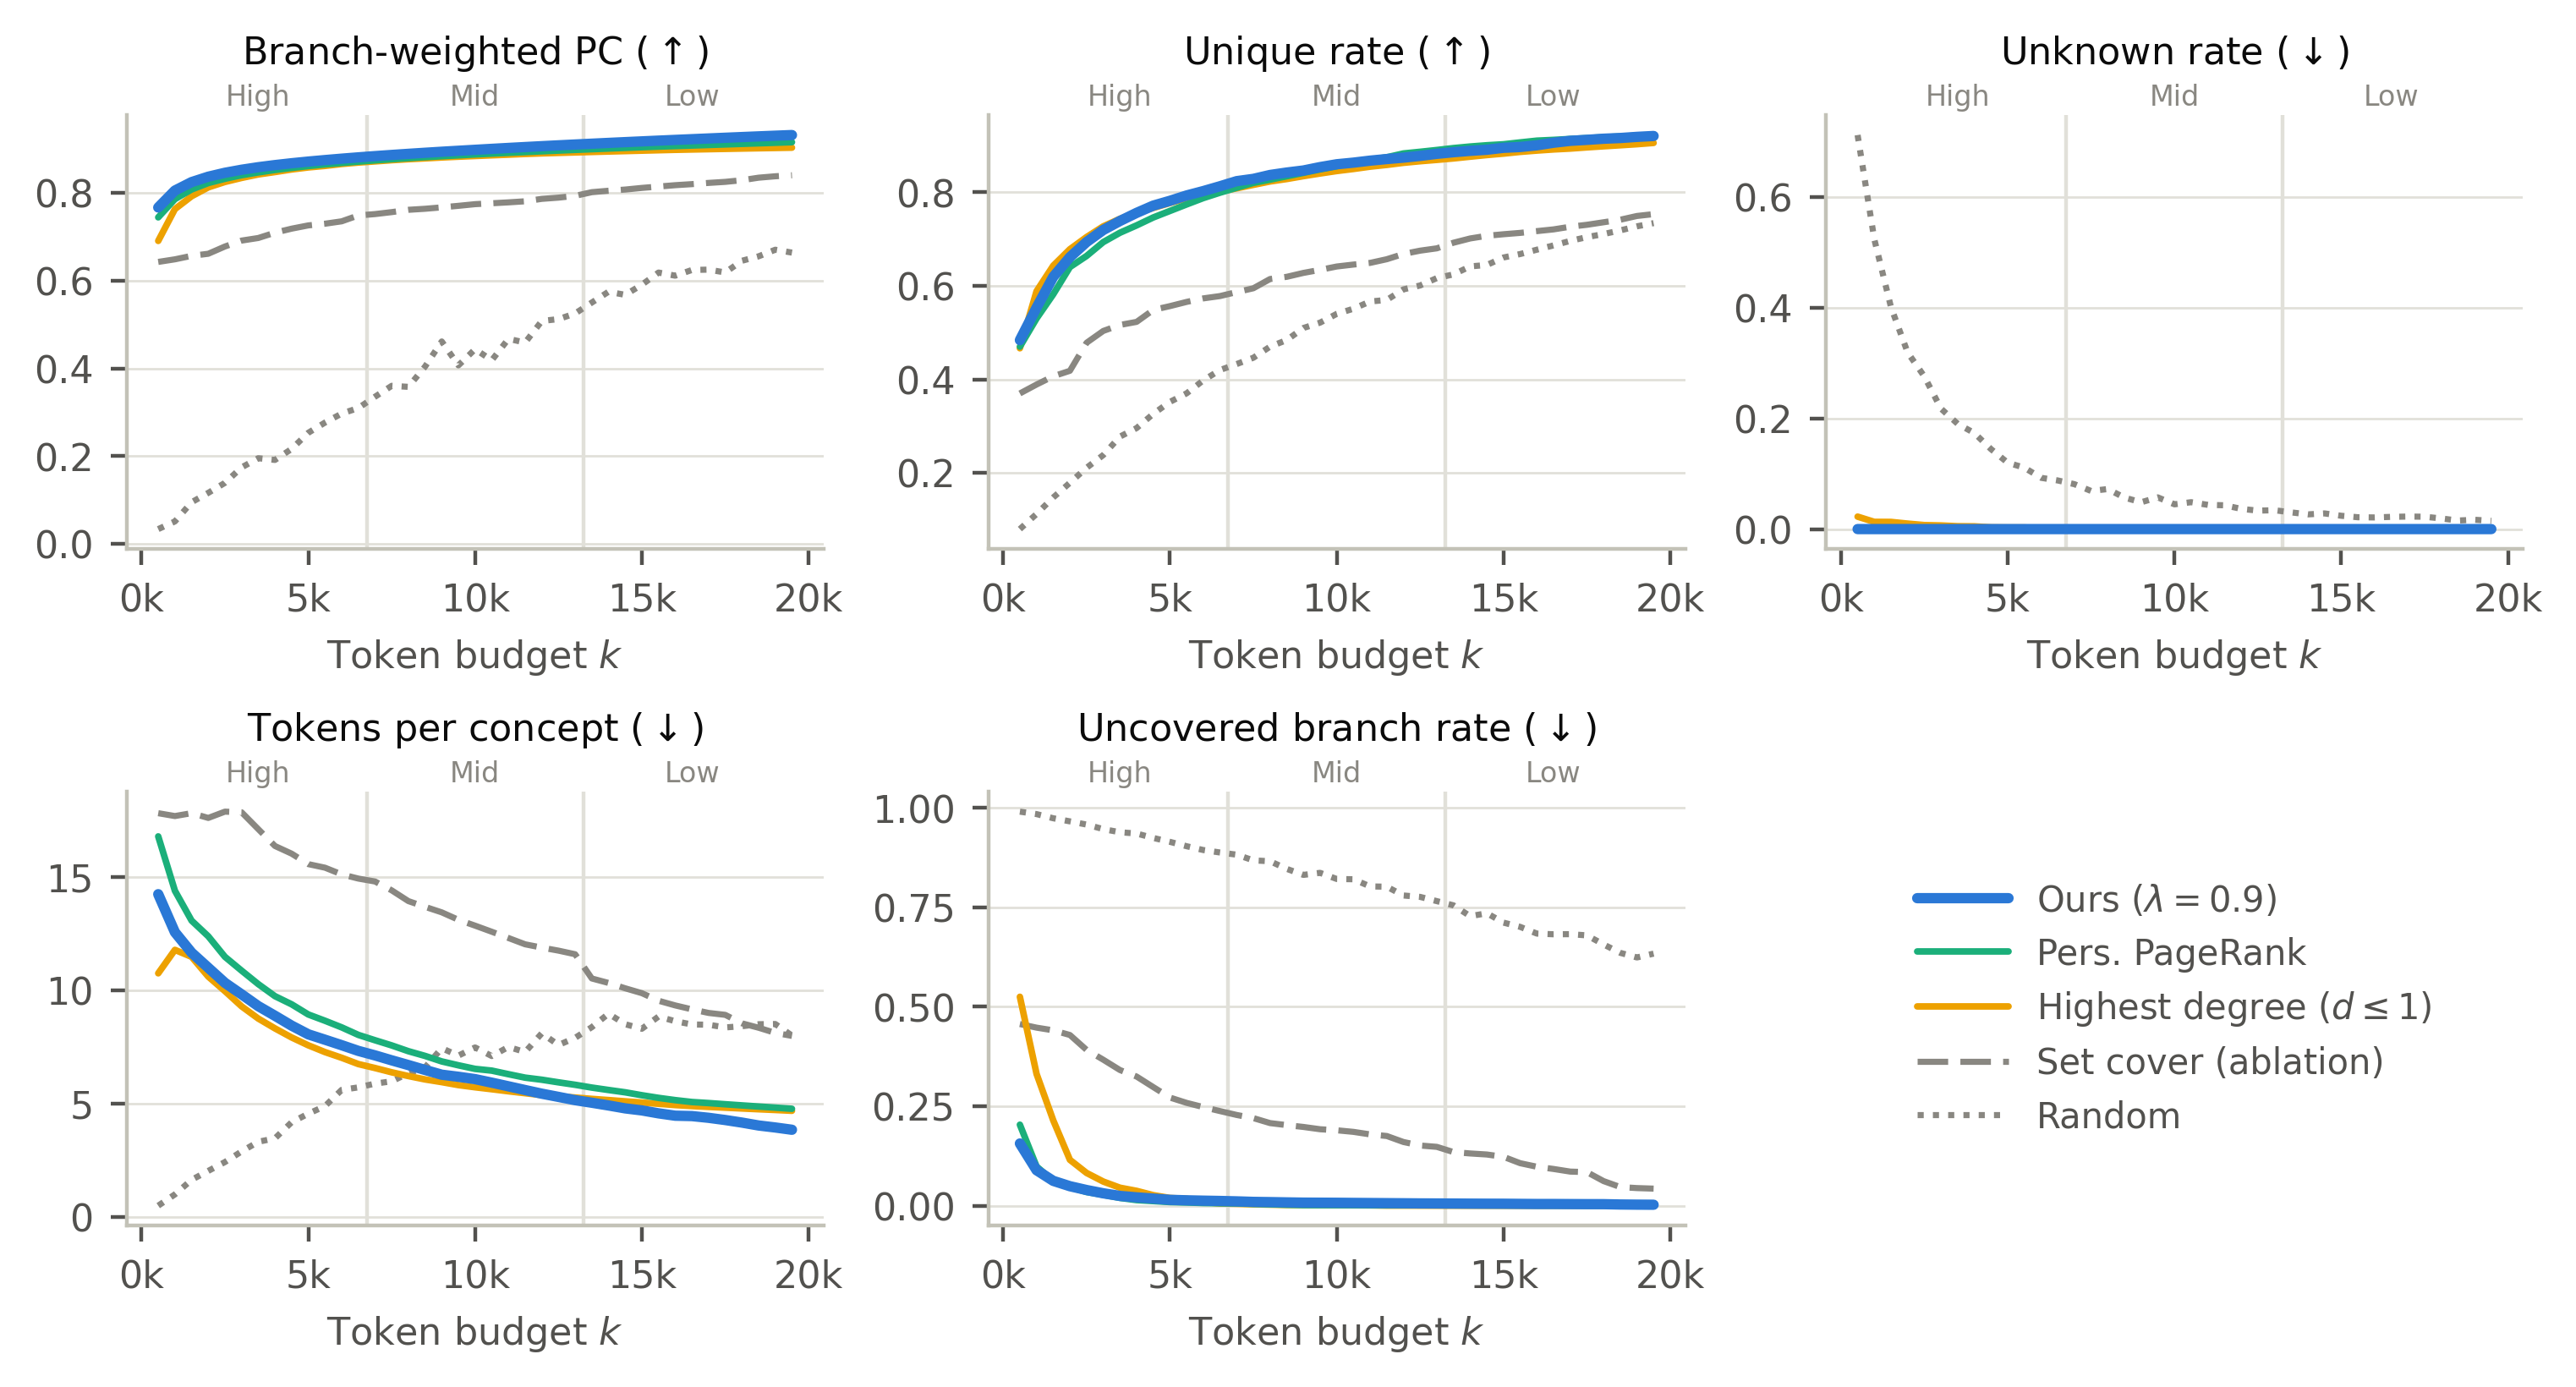
\includegraphics[width=\textwidth]{imgs/metrics_vs_k_all.png}
\caption{Core metrics as a function of the token budget $k$ for the methods of Figure~\ref{fig:metrics-vs-k}, with random selection (mean over 20 draws) added. Arrows indicate the preferred direction; vertical lines separate the high, mid and low compression levels.}
\label{fig:metrics-vs-k-all}
\end{figure*}

\section{Detailed results on the HERO data}
\label{app:hero}

Table~\ref{tab:ehr} gives the values of Figure~\ref{fig:hero} for every token budget, together with the uncovered branch rate and the share of concepts with a unique representation.
Table~\ref{tab:longtail} details, by frequency bin at $k = 5{,}000$, how much the tokens of each concept borrow events from other concepts.

\begin{table}[t]
\centering
\small
\setlength{\tabcolsep}{3.5pt}
\begin{tabular}{@{}r rr rr r rrr r r@{}}
\toprule
 & \multicolumn{2}{c}{Concepts} & \multicolumn{2}{c}{Events} & Uncov. & \multicolumn{3}{c}{Unique} & Rare, & Tokens \\
\cmidrule(lr){2-3}\cmidrule(lr){4-5}\cmidrule(lr){7-9}
$k$ & Ours & Trunc. & Ours & Trunc. & branch & Tree & Flat & Tree, ev. & tokens $\ge 10$ & per event \\
\midrule
250 & $>$99.9 & 1.5 & $>$99.9 & 82.2 & 25.8 & 51.8 & 41.9 & 21.4 & 100.0 & 9.3 \\
500 & $>$99.9 & 3.1 & $>$99.9 & 92.5 & 16.2 & 56.8 & 50.5 & 29.8 & 100.0 & 8.6 \\
1,000 & 100.0 & 6.1 & 100.0 & 97.5 & 10.3 & 62.3 & 58.7 & 41.2 & 100.0 & 7.6 \\
2,000 & 100.0 & 12.2 & 100.0 & 99.3 & 5.3 & 69.3 & 67.1 & 55.1 & 99.8 & 6.9 \\
3,500 & 100.0 & 21.4 & 100.0 & 99.8 & 2.9 & 75.1 & 73.9 & 65.3 & 97.9 & 6.0 \\
5,000 & 100.0 & 30.5 & 100.0 & 99.9 & 1.5 & 79.1 & 78.2 & 68.0 & 94.1 & 5.6 \\
7,500 & 100.0 & 45.8 & 100.0 & $>$99.9 & 0.7 & 83.9 & 83.5 & 73.3 & 85.7 & 5.2 \\
10,000 & 100.0 & 61.1 & 100.0 & $>$99.9 & 0.3 & 88.5 & 88.1 & 77.8 & 76.1 & 4.8 \\
16,370 & 100.0 & 100.0 & 100.0 & 100.0 & 0.0 & 97.3 & 97.3 & 98.5 & 51.6 & 1.8 \\
\bottomrule
\end{tabular}
\caption{Our tokenizer ($\lambda = 0.9$) and frequency truncation (Trunc.) on the HERO data; all values in \% except tokens per event.
Concepts, Events: share of the 16,370 concepts, and of the 279 million events, represented by at least one token other than the unknown token.
Uncov.\ branch: concepts whose context tree has at least one branch without a token.
Unique: concepts whose representation no other concept shares, with the context tree or with the flat token set, and the same share for the tree counted in events (Tree, ev.); under truncation, the unique shares equal the Concepts and Events columns.
Rare, tokens $\ge 10$: rare concepts (fewer than 100 events) whose every token occurs in at least 10 events.
Truncation costs one token per event; $k = |\Mhero| = 16{,}370$ keeps every concept.}
\label{tab:ehr}
\end{table}

\begin{table}[t]
\centering
\small
\setlength{\tabcolsep}{4pt}
\begin{tabular}{@{}lrrrrr@{}}
\toprule
 & Unique & \multicolumn{4}{c}{Least frequent token} \\
\cmidrule(l){3-6}
Events of the concept & tree (\%) & Events & Gain & $\ge 10$ events (\%) & No gain (\%) \\
\midrule
$< 10$ & 84.3 & 535 & 185.1 & 89.0 & 9.0 \\
$[10, 100)$ & 80.0 & 763 & 25.5 & 100.0 & 8.2 \\
$[100, 1{,}000)$ & 78.0 & 1,759 & 6.3 & 100.0 & 6.7 \\
$\ge 1{,}000$ & 66.5 & 61,017 & 3.6 & 100.0 & 7.0 \\
\bottomrule
\end{tabular}
\caption{Borrowed strength on the HERO data at $k = 5{,}000$, by number of events of the concept; the first two rows are the rare concepts.
Unique tree: concepts whose context tree no other concept shares.
Least frequent token: median number of events of the least frequent token of a concept; median ratio of this number to the concept's own number of events (gain); share of concepts whose least frequent token occurs in at least 10 events; and share with a gain of exactly 1 (no gain).
Under truncation, every kept concept has a gain of 1.}
\label{tab:longtail}
\end{table}

\section{Expert evaluation materials}
\label{app:expert}

Table~\ref{tab:expert-strata} gives the inclusion funnel and the sizes of the strata used to sample and weight the expert ratings (Section~\ref{sec:method:expert}).
\notetoself{add the rater instructions and a screenshot of the form}

\begin{table}[h]
\centering
\small
\setlength{\tabcolsep}{5pt}
\begin{tabular}{@{}llrrr@{}}
\toprule
\multicolumn{5}{@{}l}{\textit{(a) Inclusion funnel}} \\
\multicolumn{4}{@{}l}{Concepts of the HERO data} & 16,370 \\
\multicolumn{4}{@{}l}{\quad in the official SNOMED~CT release (fully defined or primitive)} & 11,796 \\
\multicolumn{4}{@{}l}{\quad\quad whose two context trees differ} & 7,490 \\
\multicolumn{4}{@{}l}{\quad\quad\quad with at most 16 tokens in the two trees together (eligible)} & 3,726 \\
\midrule
\multicolumn{5}{@{}l}{\textit{(b) Strata}} \\
Category & Status & Population & Eligible & Sampled \\
\midrule
Token in ours only & fully defined & 1,200 & 648 & 20 \\
 & primitive & 620 & 558 & 10 \\
Token in the baseline only & fully defined & 272 & 259 & 12 \\
 & primitive & 200 & 200 & 8 \\
Decomposed by both & fully defined & 3,535 & 1,023 & 34 \\
 & primitive & 1,663 & 1,038 & 16 \\
\midrule
Not rated: same tree & & 3,073 & & \\
Not rated: token in both & & 1,233 & & \\
\bottomrule
\end{tabular}
\caption{Expert evaluation: our tokenizer vs Personalized PageRank at $k = 5{,}000$ on the HERO data. Population: concepts of the official release in the stratum, used as weights. Concepts with the same tree, or kept as a token by both methods, count as ``no clear difference''.}
\label{tab:expert-strata}
\end{table}

\end{document}
